\documentclass[12pt,twoside]{article}
% above 12 pt font, even and odd pages

% !TEX root = QuickStart.tex

% add various packages and set their parameters
\usepackage{graphicx,rotate,url,mathptmx,lscape,times,framed,color}

% include natbib for bibtex, options are
% round use (2008) instead of [2008] for year
\usepackage[round]{natbib}

% cross references across documents
\usepackage{xr-hyper}

%\begin{comment}
%This is my comment.
%Note that it can span multiple lines.
%This is very useful.
%\end{comment}
\usepackage{verbatim} 

% allow hyperlinks
\usepackage{hyperref}
\hypersetup{
    bookmarks=true,         % show bookmarks bar?
    unicode=false,          % non-Latin characters in Acrobat's bookmarks
    pdftoolbar=true,        % show Acrobat's toolbar?
    pdfmenubar=true,        % show Acrobat's menu?
    pdffitwindow=true,      % page fit to window when opened
    pdftitle={My title},    % title
    pdfauthor={Author},     % author
    pdfsubject={Subject},   % subject of the document
    pdfnewwindow=true,      % links in new window
    pdfkeywords={keywords}, % list of keywords
    colorlinks=true,        % false: boxed links; true: colored links
    linkcolor=blue,         % color of internal links, def red
    citecolor=blue,         % color of links to bibliography, def green
    filecolor=blue,         % color of file links, def magenta
    urlcolor=blue           % color of external links, def cyan
}

% geometry package controls page layout
\usepackage[letterpaper,
left=2.5cm,right=2.5cm,
top=2.5cm,bottom=2.5cm]{geometry}
\oddsidemargin=+0.7cm
\evensidemargin=-0.7cm
\pagestyle{headings}

% journal name macros used by ADS
\usepackage{../common/aas_macros_v61}

% Include list of figures and references in contents lists
\usepackage[nottoc]{tocbibind}

% makes it easy to include all or part of a PDF document 
% inside a LaTeX document
\usepackage{pdfpages}

% allow external files to be included verbatim
\usepackage{moreverb}

% allow tables to wrap over pages
\usepackage{longtable}


% set the default tabsize
\def\verbatimtabsize{4\relax}

% following are to pick up .aux files for cross references
% with package xr to other volumes of Hazy
% hazy 1
\externaldocument[Hazy1-]{../hazy1/intro}[hazy1.pdf]
\externaldocument[Hazy1-]{../hazy1/define}[hazy1.pdf]
\externaldocument[Hazy1-]{../hazy1/cmdintro}[hazy1.pdf]
\externaldocument[Hazy1-]{../hazy1/cont-def}[hazy1.pdf]
\externaldocument[Hazy1-]{../hazy1/cont-lum}[hazy1.pdf]
\externaldocument[Hazy1-]{../hazy1/cont-shp}[hazy1.pdf]
\externaldocument[Hazy1-]{../hazy1/compos}[hazy1.pdf]
\externaldocument[Hazy1-]{../hazy1/density}[hazy1.pdf]
\externaldocument[Hazy1-]{../hazy1/geometry}[hazy1.pdf]
\externaldocument[Hazy1-]{../hazy1/optdepth}[hazy1.pdf]
\externaldocument[Hazy1-]{../hazy1/therm}[hazy1.pdf]
\externaldocument[Hazy1-]{../hazy1/dynamics-time}[hazy1.pdf]
\externaldocument[Hazy1-]{../hazy1/stopping}[hazy1.pdf]
\externaldocument[Hazy1-]{../hazy1/conout}[hazy1.pdf]
\externaldocument[Hazy1-]{../hazy1/optimize}[hazy1.pdf]
\externaldocument[Hazy1-]{../hazy1/grid}[hazy1.pdf]
\externaldocument[Hazy1-]{../hazy1/miscell}[hazy1.pdf]
\externaldocument[Hazy1-]{../hazy1/latex_style}[hazy1.pdf]

% hazy2
\externaldocument[Hazy2-]{../hazy2/limits}[hazy2.pdf]
\externaldocument[Hazy2-]{../hazy2/coninter}[hazy2.pdf]
\externaldocument[Hazy2-]{../hazy2/lineatomparam}[hazy2.pdf]
\externaldocument[Hazy2-]{../hazy2/linedetl}[hazy2.pdf]
\externaldocument[Hazy2-]{../hazy2/CloudyStandaloneProgram}[hazy2.pdf]
\externaldocument[Hazy2-]{../hazy2/sub}[hazy2.pdf]
\externaldocument[Hazy2-]{../hazy2/output}[hazy2.pdf]
\externaldocument[Hazy2-]{../hazy2/observed}[hazy2.pdf]
\externaldocument[Hazy2-]{../hazy2/lines}[hazy2.pdf]
\externaldocument[Hazy2-]{../hazy2/problems}[hazy2.pdf]
\externaldocument[Hazy2-]{../hazy2/odetail}[hazy2.pdf]
\externaldocument[Hazy2-]{../hazy2/sources}[hazy2.pdf]
\externaldocument[Hazy2-]{../hazy2/glossary}[hazy2.pdf]
\externaldocument[Hazy2-]{../hazy2/conversion}[hazy2.pdf]
\externaldocument[Hazy2-]{../hazy2/TestSuite}[hazy2.pdf]

% hazy 3
\externaldocument[Hazy3-]{../hazy3/isoseq}[hazy3.pdf]
\externaldocument[Hazy3-]{../hazy3/hydroiso}[hazy3.pdf]
\externaldocument[Hazy3-]{../hazy3/helikeiso}[hazy3.pdf]
\externaldocument[Hazy3-]{../hazy3/molecules}[hazy3.pdf]
\externaldocument[Hazy3-]{../hazy3/dheavy}[hazy3.pdf]
\externaldocument[Hazy3-]{../hazy3/dtherm}[hazy3.pdf]
\externaldocument[Hazy3-]{../hazy3/dgrain}[hazy3.pdf]
\externaldocument[Hazy3-]{../hazy3/dother}[hazy3.pdf]

% set paragraph styles
\raggedright
\setlength{\parindent}{4mm}
% background color for shaded boxes
\definecolor{shadecolor}{gray}{0.9}

% Customize contents details from book.cls
\makeatletter

\renewcommand*\l@section{\@dottedtocline{1}{1.5em}{3.1em}}
\renewcommand*\l@subsection{\@dottedtocline{2}{4.6em}{4.1em}}
\renewcommand*\l@subsubsection{\@dottedtocline{3}{8.7em}{5.1em}}
\renewcommand*\l@paragraph{\@dottedtocline{4}{10em}{6em}}
\renewcommand*\l@subparagraph{\@dottedtocline{5}{12em}{7em}}
\renewcommand*\l@figure{\@dottedtocline{1}{1.5em}{3.3em}}

% extract name of target of reference (e.g. chapter titles)
\long\def\@thirdoffive#1#2#3#4#5{#3}%
\def\refname#1{\expandafter\@setref\csname r@#1\endcsname\@thirdoffive{#1}}

% create ruler underneath page header
\advance\headheight1.2pt
\def\@oddhead{\vbox{\parindent=0pt%
\setbox0=\hbox to\textwidth{{\slshape\rightmark}\hfil\thepage}%
\dimen0=4.5pt \advance\dimen0 by-\dp0 \box0\kern\dimen0\hrule}}
\def\@evenhead{\vbox{\parindent=0pt%
\setbox0=\hbox to\textwidth{\thepage\hfil\slshape\leftmark}%
\dimen0=4.5pt \advance\dimen0 by-\dp0 \box0\kern\dimen0\hrule}}

% modify font size for verbatim environment
\newcommand{\setverbatimfontsize}[1]{\renewcommand*\verbatim@font{#1\ttfamily}}
\renewcommand*\verbatim@font{\footnotesize\ttfamily}

% Change title of bibliography
\renewcommand\bibname{REFERENCES}
\renewcommand\contentsname{CONTENTS}
\renewcommand\listfigurename{LIST OF FIGURES}
\renewcommand\listtablename{LIST OF TABLES}
% tweak bibliograpy environment to be more like old Hazy
\def\thebibliography#1{%
\bibsection
\@mkboth{\MakeUppercase\bibname}{\MakeUppercase\bibname}%
\list{}{\setlength\labelwidth{2.5em}\leftmargin\labelwidth
\setlength\parsep{0pt}\setlength\itemsep{0.7mm plus1pt}
\setlength{\itemindent}{-\leftmargin}
\small}
\def\newblock{\hskip .11em plus .33em minus -.07em}
\sloppy
\sfcode`\.=1000\relax}
\def\endthebibliography{\endlist}


\setcounter{tocdepth}{4}

\makeatother
% End of contents customization

% 20 06 24, copied from  aastex63.cls

%% need this change so that it works correctly in tables:
{\catcode`\$=\active
\gdef\nodata{ ~$\cdots$~ }}% 

\newcommand\diameter{\ooalign{\hfil/\hfil\crcr\mathhexbox20D}}% 
\newcommand\degr{\arcdeg}% 
\newcommand\Sun{\sun}% 
\newcommand\Sol{\sun}% 
\newcommand\sun{\odot}% 
\newcommand\Mercury{\astro{\char1}}% Mercury symbol, "1" 
\newcommand\Venus{\astro{\char2}}% Venus symbol, "2" 
\newcommand\Earth{\earth}% 
\newcommand\Terra{\earth}% 
\newcommand\earth{\oplus}% 
\newcommand\Mars{\astro{\char4}}% Mars symbol, "4" 
\newcommand\Jupiter{\astro{\char5}}% Jupiter symbol, "5" 
\newcommand\Saturn{\astro{\char6}}% Saturn symbol, "6" 
\newcommand\Uranus{\astro{\char7}}% Uranus symbol, "7" 
\newcommand\Neptune{\astro{\char8}}% Neptune symbol, "8" 
\newcommand\Pluto{\astro{\char9}}% Pluo symbol, "9" 
\newcommand\Moon{\astro{\char10}}% Moon symbol, "M" 
\newcommand\Luna{\Moon}% 
\newcommand\Aries{\astro{\char11}}% 
\newcommand\VEq{\Aries}% vernal equinox (Aries) 
\newcommand\Taurus{\astro{\char12}}% 
\newcommand\Gemini{\astro{\char13}}% 
\newcommand\Cancer{\astro{\char14}}% 
\newcommand\Leo{\astro{\char15}}% 
\newcommand\Virgo{\astro{\char16}}% 
\newcommand\Libra{\astro{\char17}}% 
\newcommand\AEq{\Libra}% autumnal equinox (Libra) 
\newcommand\Scorpius{\astro{\char18}}% 
\newcommand\Sagittarius{\astro{\char19}}% 
\newcommand\Capricornus{\astro{\char20}}% 
\newcommand\Aquarius{\astro{\char21}}% 
\newcommand\Pisces{\astro{\char22}}% 
 

% some names we use
\newcommand{\Cloudy}{\textsc{Cloudy}}
\newcommand{\Hazy}{\textsc{Hazy}}
\newcommand{\cdCommand}[1]{\textbf{#1}}
\newcommand{\cdVariable}[1]{\emph{#1}}
\newcommand{\cdSectionTitle}[1]{\emph{#1}}
\newcommand{\cdFilename}[1]{\texttt{#1}}
\newcommand{\cdRoutine}[1]{\emph{#1}}
\newcommand{\cdTerm}[1]{\textbf{\emph{#1}}}
\newcommand{\cdMono}[1]{\texttt{#1}}
\newcommand{\fixit}[1]{\textbf{FIXIT: #1}}
\font\manual=manfnt at 7pt \def\dbend{\hbox{\raise0.9ex\hbox{\manual\char127\hspace{0.6em}}}}
\newcommand{\experimental}{\texorpdfstring{\dbend}{??}}

% or symbol provided by Will H
\newcommand\OR{\texorpdfstring{\ensuremath{\vert}}{|}}

% Matt's 1.23\e{-2} 
\providecommand{\e}[1]{\ensuremath{\times 10^{#1}}}


% \ion from Will, replace AAS version
\newcommand\Ion[2]{\ensuremath{\mathrm{#1\,\scriptstyle #2}}}

% macro sometimes found in ADS bibtex entries
\newcommand{\mdash}{---} 

% ion is in the aas style
\newcounter{INTERNALionstage}
\providecommand{\ion}[2]{% replace the aastex version
  \setcounter{INTERNALionstage}{#2}%
  \Ion{#1}{\Roman{INTERNALionstage}}}

\providecommand{\red}[1]{{\color{red}#1}}

% Will's todo and done macros
%\newcommand\TODO[1]{\textbf{\boldmath [#1]}}
\newcommand{\TODO}[1]{\textcolor{red}{{\textbf{\boldmath [#1]}}}}
\newcommand\DONE[1]{{\color{green!50!gray} \textbf{DONE}} {\color{white!80!black!80!green} #1}}

\newcommand{\Av}{A$_{\rm V}$}

\def\gtsim{\mathrel{\hbox{\rlap{\hbox{\lower4pt\hbox{$\sim$}}}\hbox{$>$}}}}
\def\lesssim{\mathrel{\hbox{\rlap{\hbox{\lower4pt\hbox{$\sim$}}}\hbox{$<$}}}}
\def\Msunpyr{M$_{\odot}\,$yr$^{-1}$}
\def\Msun{M$_{\odot}$}
%       Based on PATs UNITS.TEX with some additions
%
%       Simple units
%
\def\A{{\rm\thinspace \AA}}
\def\cm{{\rm\thinspace cm}}
\def\as{{\rm\thinspace arcsec}}
\def\erg{{\rm\thinspace erg}}
\def\eV{{\rm\thinspace eV}}
\def\g{{\rm\thinspace g}}
\def\ga{{\rm\thinspace gauss}}
\def\hr{{\rm\thinspace hr}}
\def\Hz{{\rm\thinspace Hz}}
\def\K{{\rm\thinspace K}}
\def\keV{{\rm\thinspace keV}}
\def\km{{\rm\thinspace km}}
\def\kpc{{\rm\thinspace kpc}}
\def\Lsun{\mbox{$\rm\thinspace L_{\odot}$}}
\def\m{{\rm\thinspace m}}
\def\MeV{{\rm\thinspace MeV}}
\def\mJy{{\rm\thinspace mJy}}
\def\micron{\hbox{$\mu$m}}
\def\Mpc{{\rm\thinspace Mpc}}
\def\Msun{\mbox{$\rm\thinspace M_{\odot}$}}
\def\nm{{\rm\thinspace nm}}
\def\pc{{\rm\thinspace pc}}
\def\ps{{\rm\thinspace s^{-1}}}
\def\pcc{{\rm\thinspace cm^{-3}}}
\def\Ryd{{\rm\thinspace Ryd}}
\def\s{{\rm\thinspace s}}
\def\sr{{\rm\thinspace sr}}
\def\W{{\rm\thinspace W}}
\def\yr{{\rm\thinspace yr}}
%
%       Compound units
%
\def\keVscm{\mbox{$\keV\cm^{2}\,$}}
\def\cmps{\mbox{$\cm\s^{-1}\,$}}
\def\cmpss{\mbox{$\cm\s^{-2}\,$}}
\def\ccmps{\mbox{$\cm^{3}\s^{-1}\,$}}
\def\ergpccmps{\mbox{$\erg\cm^{-3}\s^{-1}\,$}}
\def\ergpg{\mbox{$\erg\g^{-1}\,$}}
\def\ergpscm{\mbox{$\erg\cm^{-2}\,$}}
\def\ergpscmps{\mbox{$\erg\cm^{-2}\s^{-1}\,$}}
\def\ergpscmpspsas{\mbox{$\erg\cm^{-2}\s^{-1}\as^{-2}\,$}}
\def\ergpscmpspa{\mbox{$\erg\cm^{-2}\s^{-1}\A^{-1}\,$}}
\def\ergps{\mbox{$\erg\s^{-1}\,$}}
\def\gpcm{\mbox{$\g\cm^{-3}\,$}}
\def\gpcmps{\mbox{$\g\cm^{-3}\s^{-1}\,$}}
\def\gps{\mbox{$\g\s^{-1}\,$}}
\def\uJy{\mbox{$\mu${\rm Jy}}}
\def\kmps{\mbox{$\km\ps\,$}}
\def\kmpspMpc{\mbox{$\kmps\Mpc^{-1}\,$}}
\def\Lsunppc{\mbox{$\Lsun\pc^{-3}\,$}}
\def\Msunpc{\mbox{$\Msun\pc^{-3}\,$}}
\def\Msunpkpc{\mbox{$\Msun\kpc^{-1}\,$}}
\def\Msunppc{\mbox{$\Msun\pc^{-3}\,$}}
\def\Msunppcpyr{\mbox{$\Msun\pc^{-3}\yr^{-1}\,$}}
\def\Msunpyr{\mbox{$\Msun\yr^{-1}\,$}}
\def\Msunpyrpkpc{\mbox{$\Msun\yr^{-1}\kpc^{-1}\,$}}
\def\ps{\mbox{$\s^{-1}\,$}}
\def\pscm{\mbox{$\cm^{-2}\,$}}
\def\psm{\mbox{$\m^{-2}\,$}}
\def\pccm{\mbox{$\cm^{-3}\,$}}
\def\pscm{\mbox{$\cm^{-2}\,$}}
\def\pscmps{\mbox{$\cm^{-2}\, \s^{-1}\,$}}
\def\pcm{\mbox{$\m^{-3}\,$}}
\def\pccmK{\mbox{$\cm^{-3}\K$}}
\def\pcmK{\mbox{$\m^{-3}\K$}}
\def\pressure{\mbox{$\g\, \cm^{-1}\, \s^{-2}\,$}}
\def\pyr{\mbox{$\yr^{-1}\,$}}
\def\pyrppc{\mbox{$\yr^{-1}\pc^{-1}\,$}}
\def\scm{\mbox{$\cm^{2}\,$}}
\def\Wpsm{\mbox{$\W\psm\,$}}
\def\Wpscm{\mbox{$\W\pscm\,$}}
\def\WHz{\mbox{$\W\Hz\,$}}
%
% spectral lines
%
\def\la{\mbox{{\rm L}$\alpha$}}
\def\pa{\mbox{{\rm P}$\alpha$}}
\def\ha{\mbox{{\rm H}$\alpha$}}
\def\hb{\mbox{{\rm H}$\beta$}}
\def\hi{\mbox{{\rm H~{\sc i}}}}
\def\hii{\mbox{{\rm H~{\sc ii}}}}
\def\hei{\mbox{{\rm He~{\sc i}}}}
\def\heii{\mbox{{\rm He~{\sc ii}}}}
\def\ci{\mbox{{\rm C~{\sc i}}}}
\def\cii{\mbox{{\rm C~{\sc ii}}}}
\def\ciii{\mbox{{\rm C~{\sc iii}}}}
\def\civ{\mbox{{\rm C~{\sc iv}}}}
\def\ni{\mbox{{\rm N~{\sc i}}}}
\def\nii{\mbox{{\rm N~{\sc ii}}}}
\def\oi{\mbox{{\rm O~{\sc i}}}}
\def\oii{\mbox{{\rm O~{\sc ii}}}}
\def\oiii{\mbox{{\rm O~{\sc iii}}}}
\def\neii{\mbox{{\rm Ne~{\sc ii}}}}
\def\neiii{\mbox{{\rm Ne~{\sc iii}}}}
\def\nev{\mbox{{\rm Ne~{\sc v}}}}
\def\mgii{\mbox{{\rm Mg~{\sc ii}}}}
\def\cliii{\mbox{{\rm Cl~{\sc iii}}}}
\def\sii{\mbox{{\rm S~{\sc ii}}}}
\def\siii{\mbox{{\rm S~{\sc iii}}}}
\def\ariii{\mbox{{\rm Ar~{\sc iii}}}}
\def\caii{\mbox{{\rm Ca~{\sc ii}}}}
\def\fei{\mbox{{\rm Fe~{\sc i}}}}
\def\feii{\mbox{{\rm Fe~{\sc ii}}}}
\def\feiii{\mbox{{\rm Fe~{\sc iii}}}}
\def\feiv{\mbox{{\rm Fe~{\sc iv}}}}
\def\fev{\mbox{{\rm Fe~{\sc v}}}}
\def\fevi{\mbox{{\rm Fe~{\sc vi}}}}
\def\fevii{\mbox{{\rm Fe~{\sc vii}}}}
\def\feviii{\mbox{{\rm Fe~{\sc viii}}}}
\def\feix{\mbox{{\rm Fe~{\sc ix}}}}
\def\fex{\mbox{{\rm Fe~{\sc x}}}}
\def\fexi{\mbox{{\rm Fe~{\sc xi}}}}
\def\fexii{\mbox{{\rm Fe~{\sc xii}}}}
\def\fexiii{\mbox{{\rm Fe~{\sc xiii}}}}
\def\fexiv{\mbox{{\rm Fe~{\sc xiv}}}}
\def\fexv{\mbox{{\rm Fe~{\sc xv}}}}
\def\fexvi{\mbox{{\rm Fe~{\sc xvi}}}}
\def\fexvii{\mbox{{\rm Fe~{\sc xvii}}}}
\def\fexviii{\mbox{{\rm Fe~{\sc xviii}}}}
\def\fexix{\mbox{{\rm Fe~{\sc xix}}}}
\def\fexx{\mbox{{\rm Fe~{\sc xx}}}}
\def\fexxi{\mbox{{\rm Fe~{\sc xxi}}}}
\def\fexxii{\mbox{{\rm Fe~{\sc xxii}}}}
\def\fexxiii{\mbox{{\rm Fe~{\sc xxiii}}}}
\def\fexxiv{\mbox{{\rm Fe~{\sc xxiv}}}}
\def\fexxv{\mbox{{\rm Fe~{\sc xxv}}}}
\def\fexxvi{\mbox{{\rm Fe~{\sc xxvi}}}}
%
% types of baryons
\def\water{\mbox{{\rm H}$_2${\rm O}}}
\def\CO{\mbox{{\rm CO}}}
\def\OH{\mbox{{\rm OH}}}
\def\htwo{\mbox{{\rm H}$_2$}}
\def\hone{\mbox{{\rm H}$^0$}}
\def\h0{\mbox{{\rm H}$^0$}}
%
% \def\H{\mbox{{\rm H}}}
%
\def\hplus{\mbox{{\rm H}$^+$}}
\def\hminus{\mbox{{\rm H}$^-$}}
% cannot have numbers in names, so cap Oh represents zero
\def\hO{\mbox{{\rm H}$^0$}}
\def\heO{\mbox{{\rm He}$^0$}}
\def\heo{\mbox{{\rm He}$^0$}}
\def\heplus{\mbox{{\rm He}$^+$}}
\def\hePP{\mbox{{\rm He}$^{2+}$}}
\def\cO{\mbox{{\rm C}$^0$}}
\def\cplus{\mbox{{\rm C}$^+$}}
%
\def\Hrec{\mbox{${\rm H}_{rec}$}}
%\def\Hrec{\mbox{$H_{rec}$}}
\def\centreline{\centerline}
%
% Nina
\DeclareMathAlphabet{\vib}{OML}{cmm}{m}{it}
% From Glenn
\newcommand*{\satellite}[1]{\textit{#1}}
\newcommand*{\xmm}{\satellite{XMM-Newton}}
\newcommand*{\chandra}{\satellite{Chandra}}
\newcommand*{\asca}{\satellite{ASCA}}
\newcommand*{\rosat}{\satellite{ROSAT}}
\newcommand*{\prog}[1]{\textsc{#1}}
%% For kb, mH. etc. Italic with non-italic subscript.
\newcommand*{\mysub}[2]{\ensuremath{#1_{\mathrm{#2}}}}

%
% this is a list of the macros the word version of hazy knew about
% these were dynamic links to the values in the code
%
% these have been incorporated in the latex
% most of the names had underscores and were in ALL CAPS
% latex does not like this, so CamelCase is used instead

% current version of Cloudy
\def\VERSION{23} 

% in cddefines.h
\def\LIMELM{30} % number of elements

% these are in phycon.h
\def\TEMPLIMITLOW{{$2.8 \K$}}    % lowest allowed temperature
\def\TEMPLIMITHIGH{{$1.001 \times 10^{10} \K$}}   % highest allowed temperature
\def\TEMPSTOPDEFAULT{{$4000 \K$}} % default stop temperature

% rfield.h
\def\emm{{$3.040 \times 10^{-9} \Ryd$}} %low energy limit to continuum in Ryd
\def\emmmhz{{10~MHz}} %low energy limit to continuum in MHz
\def\emmcm{{29.98 m}} %low energy limit to continuum in meters

\def\egamry{{$7.354\times 10^6 \Ryd$}} %high energy limit to continuum in Ryd
\def\egamrymev{{$100 \MeV$}} %high energy limit to continuum in MeV

% feii.h
% short, long wavelength limits of save feii continuum,
% and number of cells to break this into
% changed with set feii continuum command

\def\speciesConWlLo{{1000 \AA}} % short wavelength limit
\def\speciesConWlHi{{7000 \AA}} % long wavelength limit
\def\speciesConNbins{{1000}} % number of bins

\def\FeIIfeconwlLo{{1000 \AA}} % short wavelength limit
\def\FeIIfeconwlHi{{7000 \AA}} % long wavelength limit
\def\FeIInfecon{{1000}} % number of bins

% default error, changed with MONITOR SET ERROR
\def\ErrorDefault{{0.05}}
% default performance monitor, changed with MONITOR SET PERFORMANCE ERROR
\def\ErrorDefaultPerformance{{0.2}}

%conv.h
%fraction convergence on iterate to convergence command
\def\autocv{{0.20}} 

%atmdat.h
%Default limits for the number of levels to use
\def\nDefaultPhotoLevelsFe{{25}}
\def\nDefaultPhotoLevels{{15}}
\def\nDefaultCollLevelsFe{{100}}
\def\nDefaultCollLevels{{50}}
\def\nDefaultMolLevels{{70}}
\def\nDefaultResLevelsHlike{{10}}
\def\nDefaultColLevelsHlike{{15}}
\def\nDefaultResLevelsHlikeall{{5}}
\def\nDefaultColLevelsHlikeall{{2}}
%nhlvl	15	default number of levels in H atom
%nhydro_small_level	10	Number of h levels with small option
%nhydro_large_level	50	Number of h levels with large option
%NHYDRO_MAX_LEVEL	400	Largest possible number of H levels
\def\nHydroMaxLevel{{400}}
\def\INPUTLINELENGTH{{2000}}
\def\LabelLenMax{{9}}

% variables above this line have been converted in all three volumes of hazy

% these have not
%BackgroundT	2.725	Temperature of background
%BackgroundTError	0.002	Uncertainty in tempeature of background
%C12_C13_isotope_ratio	30	C12 / C13 isotope ratio
%capots	1.5	
%colend	1030 cm-2	
%colpls	1030 cm-2	
%colnut	1030 cm-2	
%cylind	1035 cm	
%D2H_ratio	1.65  times10-5	Deuterium to hydrogen abundance ratio
%date	09.02
%Field giving date in format yy.mm
%didz	0.15	optical depth at interaction max, used for nextdr
%ehixray	100 keV	highest energy called "x-ray"
%EdenError	0.01	error in electron density
%faint	10-3	
%flxfnt	10-10	
%hazy	HAZY	
%H2_to_H_limit	10-8	Smallest H2/H ratio where large H2 mole computed, %in h2
%nIterOptim	20	limit to number off iterations, optimizer
%limfal	20	limit to number of thermal failures
%limLevelN	20	limit to number of levels in leveln
%limspc	100	limit to number of continua with table/interpolate
%limTabD	500	limit to number of pairs in dlaw table command
%limpar	20	limit to number of parameters to vary
%line_length	200	limit to length of input line
%lmhlvl	400	limit to number of levels of H atom
%lyman_extra	100	Number of extra lyman line in iso atoms
%ncell	130000	dimension of continuum arrays
%ndust	500	Limit number of grains bins
%Ndplot	10	number of plots
%limelm	30	total number of elements
%limpun	100	limit to number of save comnd
%NCOROTATE	20	Default number of CO rotation levels
%nelemMH	29	number of elem, minus H
%nend	1400	limit to number of zones, nEndDflt in code
%nFe2LevN	371	number of levels in large FeII atom
%n_initial_relax	2	Number of iterations to relax dynamical %calculation
%NCOLLM	100	Number of column den in optimize cod
%nlines	106	number of emission lines
%nobslm	100	limit to number of observations in vary
%npunlm	100	limit to number of lines in save lines cum struc
%nrdsum	30	lim to #lines in stoy sum
%Optim_def_error	0.05	Default error on quantities in optimization %cmnd
%PressureError	0.01	Largest relative error in pressure
%PrtTauFnt	0.1	faintest line tau to print
%Resolution	matched to Cloudy mesh	Resolution for save file contrast
%rdfalt	1030 cm	default inner radius
%router	1031 cm	default outer radius
%toler	0.005	Fractional error in heating-cooling mismatch
%tsqden	107 cm-3	highest value to print Peimbert analysis of t2
%vtoler	0.10	default tolerance for optimizer
%mxstpl	10	number of stop line commands
%nmaps	20	number of steps in heating cooling map
%WeakHeatCool	0.05	Faintest heating or cooling agent to save, set %with set WeakHeatCool command


\begin{document}
%\frontmatter

%%%%%%%%%%%%%%%%%%%%%%%%%%%%%%%%%%%%%%%%%%%%%%%
%  title page
\begin{titlepage}
\begin{center}

\Huge
\emph{Quick Start Guide to \Cloudy\ C\VERSION}\\
\begin{figure}
\begin{center}

\includegraphics[clip=on,width=\columnwidth,height=0.7\textheight,keepaspectratio]{cycling_race.jpg}
\end{center}
\label{fig:header}
\end{figure}

\LARGE

\vspace{15 mm }
\LARGE
\emph{Cloudy \& Associates} \\
\Large
\href{http://www.nublado.org}{www.nublado.org} \\
\normalsize
\today
\end{center}
\end{titlepage}

%%%%%%%%%%%%%%%%%%%%%%%%%%%%%%%%%%%%%%%%%%%%%%%
% page with one figure and boilerplate text
\clearpage
{\small
\noindent
{\em Software:} Copyright \copyright\ 1978-2023 Gary J. Ferland and others. All rights reserved.

\vspace{1em}

\noindent
The software described in this documentation (\Cloudy) is subject
to a FreeBSD-style software license
contained in the file \cdFilename{license.txt} in the
root directory of the distributed files.
The list of co-authors is given in the file
\cdFilename{others.txt} in the same directory.
Use of this program is not restricted provided each use is
acknowledged upon publication.
The bibliographic reference to this version of \Cloudy\ is
``version xx.xx
of the code last described \citet{CloudyReview}.''
The version number, shown here as ``xx.xx'', should be
given.
This version number, along with a complete citation,
can be found by executing the code with the 
\cdCommand{print citation} command included in the input script.

\vspace{1em}

\noindent
\Cloudy\ is an evolving code.
You should confirm that you have the most recent
version of the code by checking the web site
\href{http://www.nublado.org}{www.nublado.org}.
The code has a
\href{https://cloudyastrophysics.groups.io}{discussion board} with emailing list.
This will have announcements of any updates to the code.\par

\vspace{1em}

\noindent
Portions of the documentation have been published, and are copyrighted by, the
American Astronomical Society, the Astronomical Society of the Pacific, and
the Royal Astronomical Society. The remainder of the documentation is subject
to the following FreeBSD format documentation license:

\vspace{1em}

\noindent
{\em Documentation:} Copyright \copyright\ 1978--2023 Gary J. Ferland and others. All rights reserved.

\vspace{1em}

\noindent
Redistribution and use of the documentation (all parts of \Hazy\ and the
Quick Start Guide) in source (\LaTeX) and `compiled' forms (PDF, PostScript,
HTML and so forth) with or without modification, are permitted provided that
the following conditions are met:

\begin{enumerate}
\item
Redistributions of source code (\LaTeX) must retain the above copyright notice,
this list of conditions and the following disclaimer as the first lines of
the file \cdFilename{license\_doc.txt} in the root directory unmodified.
\item
Redistributions in compiled form (converted to PDF, PostScript, XML, HTML and
other formats) must reproduce the above copyright notice, this list of
conditions and the following disclaimer in the documentation and/or other
materials provided with the distribution.
\end{enumerate}

\noindent
{\em This documentation is provided by the \Cloudy\ project ``as is'' and any express
or implied warranties, including, but not limited to, the implied warranties
of merchantability and fitness for a particular purpose are disclaimed. In no
event shall the  \Cloudy\  project be liable for any direct, indirect, incidental,
special, exemplary, or consequential damages (including, but not limited to,
procurement of substitute goods or services; loss of use, data, or profits; or
business interruption) however caused and on any theory of liability, whether
in contract, strict liability, or tort (including negligence or otherwise)
arising in any way out of the use of this documentation, even if advised of
the possibility of such damage.}\par
}

\vspace{5mm}
\noindent
{\small
{\em Cover image:}
Bavarian Road Cycling Championship 2017, in Baiersdorf (Middle Franconia).
Photo by
\href{https://unsplash.com/@markusspiske}{Markus Spiske} on
\href{https://unsplash.com/license}{Unsplash}.
\clearpage

%%%%%%%%%%%%%%%%%%%%%%%%%%%%%%%%%%%%%%%%%%%%%%%
%  table of contents - only include top two levels
\setcounter{tocdepth}{2}
\tableofcontents

\clearpage

\section{Introduction}
\label{sec:Introduction}

Numerical simulations make it
possible to understand complex physical
environments starting from first principles.  Cloudy is designed to do just
that.  It determines the physical conditions within a non-equilibrium gas,
possibly exposed to an external source of radiation, and predicts the
resulting spectrum.  This makes it possible to predict many observed
quantities by specifying only the properties of the cloud and the radiation
field striking it.

This is a quick-start guide to Cloudy.  It begins with an introduction
to the code's web site, outlines how to set up the code, and is followed
by a description of \Hazy, the code's documentation.  This document only
gives an outline of the code and the commands that drive it.  Sections of
\Hazy\ that go into greater detail are referenced and should be consulted
to find out more.

Osterbrock \& Ferland (2006; hereafter AGN3) give many more details
about photoionized clouds.
This is an active research field.
\citet{Ferland03} reviews recent advances and
current questions.

\subsection{The web site and discussion board}

Cloudy is open source.  Its source, atomic data files, a large suite
of test cases, and its documentation \Hazy, are available at the web site
\href{http://www.nublado.org}{www.nublado.org}.
Begin setting up the code by going to the
web site and
follow the instructions under
\emph{Instructions for downloading and installing the release version }.

The web site includes a link to a 
\href{https:cloudyastrophysics.groups.io}{discussion board}.  This is the place
to ask questions, make suggestions, and report problems.

The following are among the most useful pages on the web site:
%
\begin{itemize}

\item 
\href{https://gitlab.nublado.org/cloudy/cloudy/-/wikis/StepByStep}
     {Download and setup the code}

\item
\href{https://gitlab.nublado.org/cloudy/cloudy/-/wikis/Frequently-asked-Questions-about-Cloudy}
     {Cloudy's Frequently Asked Question page}

\item
\href{https://cloudyastrophysics.groups.io}{The discussion group}

\item
\href{https://gitlab.nublado.org/cloudy/cloudy/-/wikis/DownloadLinks}
     {Just download the code and its documentation}

\item
\href{https://gitlab.nublado.org/cloudy/cloudy/-/wikis/RevisionHistory}
     {A list of improvements to the code}

\item
\href{https://gitlab.nublado.org/cloudy/cloudy/-/wikis/KnownProblems}
     {Known problems with the code}

\item
\href{https://gitlab.nublado.org/cloudy/cloudy/-/wikis/HotFixes}
     {Hot fixes, small changes to the code that fix bugs}
\end{itemize}

\subsection{The release version}

Like all software, Cloudy goes through versions as it is developed.
The fidelity of the simulation improves as processors become faster.  Atomic
and molecular rate coefficients become better as theory and experiment makes
progress.  Bugs are fixed.
As a result the code goes through versions and its predictions improve over time.

The \cdTerm{release version} should
be used for all publications.  Papers
should say exactly what version of the code was used.
All versions of Cloudy
that ever have been the release version are still on the web site.
This makes it possible to reproduce results obtained years ago should a
question about results ever arise.

Several development versions are also on the web site and in the
subversion repository.  These are experimental and should not be used in
published work.

New versions of the code, and patches to the current version, are
announced on  
\href{https://cloudyastrophysics.groups.io}{cloudyastrophysics.groups.io}.

\subsection{\Hazy, the documentation}

Cloudy's documentation \Hazy\ comes in four volumes.
This \emph{Quick Start Guide} gives an overview.
Part 1 gives a complete list of all commands.
Part 2 describes the output that is generated, shows how to extract
observed quantities from the predictions, and explains how to call Cloudy
as part of a larger program.  
The \emph{Quick Start Guide}, and Parts 1 and 2, are kept up to date and PDF versions are included
in the download in the directory \cdFilename{cloudy/docs}.

Part 3, which is badly out of date at the time of this writing, describes
the physics behind the simulation.  The past few years have seen many
expansions of the code's capabilities, especially in infrared emission,
molecular physics, dynamics and advective flows,
and time dependent simulations.
Unfortunately, Part 3 of \Hazy\ has not had a high enough
priority to be updated with available resources.  I have not given up and
do intend to update this section eventually.  For now, an ADS search on
\href{http://adsabs.harvard.edu/cgi-bin/abs_connect?author=ferland\%2C+g&amp;return_req=no_params}{Ferland} will find the most recent papers that describe advances in the
physics.

The \LaTeX\ source needed to build the documentation is included in \cdFilename{cloudy/docs/latex}.
The Perl script \cdFilename{CompileAll.pl} will compile all four parts of the documentation,
leaving PDF files in the appropriate subdirectories.

\subsection{Assumptions}

The code computes the non-equilibrium ionization, thermal, and chemical
state of a cloud that may (or may not) be exposed to an external source
of radiation.  The usual assumption is that atomic processes have had time
to become time steady.  The density of a species or level i is given by
a balance equation of the form
\begin{equation}
\frac{\partial n_i}{\partial t} = \sum_{j \ne i} n_j R_{ji} +
  Source - n_i \left( \sum_{ji} R_{ij}  + Sink \right) = 0
  \ \rm{[cm^{-3} \, s^{-1}]}
\end{equation}
Here $R_{ji}$ represents the rate [s$^{-1}$] that a species $j$ goes to $i$,
$Source$ is
the rate per unit volume [cm$^{-3}$ s$^{-1}$]
that new atoms appear in $i$, and $Sink$
is the rate [s$^{-1}$] they are lost.  This,
together with equations representing
conservation of energy, mass, and charge, fully specify the problem.

Most calculations assume that the cloud is static.
The ability to do dynamical and time-dependent calculations is
now in the code although this part is not fully mature.
\citet{HenneyEtAl05} and \citet{HenneyEtAl07} present
examples of dynamical calculations.

The \cdTerm{Introduction} chapter in \Hazy\ Part 1 gives more details on the assumptions.
The section \cdTerm{The Future} on \href{http://www.nublado.org}{www.nublado.org}
outlines the directions future development will take.
ALI line radiative transfer and expansion to two and three dimensional geometries
are some of the planned future development.

\subsection{What Cloudy can do}

Given these assumptions the code will determine the ionization,
temperature, and chemical state of a cloud and then predict its spectrum.
All of this is done self-consistently with the minimum number of free
parameters.

The equations of statistical equilibrium, charge conservation, and
conservation of energy are solved.  These determine the level of ionization,
the particle density, the gas kinetic temperature, the chemical state,
populations of levels within atoms, and the full spectrum, which often
includes hundreds of thousands of lines.  A very large number of observables
result from a very few free parameters.  Often the goal is to determine these
free parameters from observations.  This approach is outlined in Section
8 of \citet{Ferland03}.

The following sections outline how to set up the boundary conditions
for a calculation.  You create an input script that specifies the cloud's
geometry, composition, density, and thickness.  The radiation field striking
the cloud, often its only source of heat and ionization, is specified, and
other sources of heat can also be included.  The code then computes the
thermal, ionization, and chemical properties of the cloud, and its observed
spectrum.  A general introduction to such environments is given in
Chapters~1 and~2 of AGN3.  The first chapter
of Part~1 of \Hazy\ gives a more extensive
overview of the code.
The format of the input script, the file that
specifies the boundary conditions, is described in the chapter
\cdTerm{Introduction to Commands} of Part~1 of \Hazy.
Output options are described in the
chapter \cdTerm{Controlling Output} of Part~1 of \Hazy.

\subsection{Definitions}

There is a fair amount of jargon that goes along with quantitative
spectroscopy and numerical simulations of a cloud.  These are summarized
in the chapter \cdTerm{Definitions} of Part~1 of \Hazy\ and in Chapters~1 through~5
of AGN3.  As a minimum you should know the definitions of the two types of
geometries (open and closed), the radiation field (incident, transmitted, diffuse,
and reflected), and the terms covering factor, density, and column density.
The Rydberg unit of energy is commonly used in this field.
Many astronomers do not understand the distinction between
\hO\ and \hi .
Don't be one of them!  The difference is significant and is given
on the web site.

\subsection{Citing the use of \Cloudy}

Publications should cite the code by giving the version number and a
reference to the last major review of Cloudy's development,
\citet{CloudyReview}.
An example would be ``We used version 07.02.01 of Cloudy, last
described by \citet{CloudyReview}.''
Citations are important for sustaining the development of Cloudy.
The exact version should be given so that, years
from now, it will be possible to find how a particular result was obtained.
The command \cdCommand{print citation} will print the correct citation in a
\LaTeX-friendly format.
Please follow the citation example shown above.

\subsection{Collaborations}

Some of the most useful additions to the code have been surprises donated
by volunteers.  There is a great deal of work left to be done.  You are
welcome to help out!

\section{Two very simple models}
\label{sec:TwoVerySimpleModels}

As a simple introduction let's create two simple models.  The first is
a planetary nebula (see Chapter~10 of AGN3) and the second is a cloud in
the Broad Emission Line Region of a quasar (Chapter~13 of AGN3).  As a
minimum you must specify a few parameters.
These include the shape and luminosity of the radiation field
striking the cloud, the cloud's density, radius,
and composition (if it is not solar).
We go over these briefly here.

\subsection{What must be specified}

Cloudy needs to be able to deduce the following information before it
can predict conditions within a cloud;

\begin{itemize}
\item The shape and brightness of the radiation field striking the cloud.
\item The total hydrogen density.
\item The composition of the gas and whether grains are present.
\item The thickness of the cloud.
\end{itemize}

Unless otherwise specified the gas-phase abundances will
be close to solar values and grains will not be included.
The total hydrogen density will be kept constant across the cloud
since this is the default.
Constant pressure, hydrostatic equilibrium, wind models
and several other geometries could have been done.

The code's philosophy is for a reasonable set of conditions to be assumed
by default.
These are listed in Section~3.3 of Part~1 of \Hazy.
Commands are added to change these conditions.

\subsection{Running a model}

Each line in the input file gives a command.
These commands are described further below.
Comments can be entered in several ways, as described in
the subsection \cdTerm{Comments} in the
chapter \cdTerm{Introduction to Commands} in
Part~1 of \Hazy.
In examples below lines beginning with ``\#'' are comments.
The file ends with a blank line or the end of file.

If the executable is called \cdFilename{cloudy.exe}
then a single simulation could be run with the command
\small
\begin{verbatim}
cloudy.exe -r sim
\end{verbatim}
\normalsize
This will read from the input file \cdFilename{sim.in} and 
produce the output file \cdFilename{sim.out}. 

Alternatively you can supply the \Cloudy\ commands on the command line. This
is useful if you quickly want to execute a one- or two-line script. An example is:
\small
\begin{verbatim}
cloudy.exe -e test
\end{verbatim}
\normalsize
which will execute the command \cdCommand{test} (the ``smoke test'', see \Hazy~1
for details).

The \href{http://www.nublado.org}{www.nublado.org} web site has many more details
about running this version of \Cloudy\ in the page
\href{https://gitlab.nublado.org/cloudy/cloudy/-/wikis/RunCode}{RunCode}.

It is also possible for a larger program to drive \Cloudy\ directly by
treating it as a subroutine. 
See \href{https://gitlab.nublado.org/cloudy/cloudy/-/wikis/RunCode}{RunCode}
for more details.

\subsection{Command format}

A series of commands tell Cloudy what to do.
They are entered, one command per line,
into an input file that is read by the code.
With a few important
exceptions, the commands can be entered in any order.
Each command is
identified by the first~4 or~5 letters on the line.
The format for commands is described further in the
chapter \cdTerm{Introduction to commands} of Part~1 of \Hazy.

Parameters are specified by numbers that appear on the command line.
Many numbers are entered as logs.
It is important to read \Hazy\ to see what is
expected for numerical input.
For instance, numbers representing
temperatures are interpreted as logs if they are
less than or equal to 10 and as the linear
temperature if greater than 10.
Many commands have the keywords \cdCommand{log} and
\cdCommand{linear} to change the default interpretation of a number.

\subsection{A simple planetary nebula}

A planetary nebula is a cloud of gas and dust that has been ejected by
a dying star (see Chapter~10 of AGN3).  The temperature and luminosity of
the central star are specified since starlight is the energy source.  The
central star is a cooling white dwarf.
We approximate its radiation field as a hot blackbody
at the Eddington limit for one solar mass.  We set the stellar continuum
shape and luminosity with separate commands:
\small
\begin{verbatim}
blackbody, T=1e5 K   # the continuum shape
luminosity total 38    # the luminosity, log erg s-1
\end{verbatim}
\normalsize
The spectral energy distribution is a $10^5 \rm{K}$ blackbody
with a total luminosity of $10^{38} \rm{erg s^{-1}}$.
The \cdCommand{blackbody} command specifies the shape of the incident
radiation field and the \cdCommand{luminosity} command
specifies its brightness.
Luminosity and shape commands are described in Section~\ref{sec:IncidentRadiationField}
on page \pageref{sec:IncidentRadiationField}.
The brightness of the incident radiation field is specified
as either a luminosity or intensity as described on
page \pageref{sec:LuminosityVsIntensityCases} below.

This example specifies a luminosity so the inner radius of the cloud
must also be specified.
This is the \emph{luminosity case} described on
page \pageref{sec:LuminosityVsIntensityCases}.
A typical inner radius for the shell of a planetary nebula is a fraction
of a parsec, so let's use $10^{18} \cm$.
A typical hydrogen density, measured
from ratios of forbidden lines (AGN3 Chapter~5),
is roughly $10^5 \pcc$.
Images suggest that the gas fully covers the star so we include the
\cdCommand{sphere} command (discussed in Section~\ref{command:sphere}
on page \pageref{command:sphere}).
A solar chemical composition would be used if we didn't change it.
The composition of
the ejected gas has been affected by nuclear processing and
dust formed during late stages of mass loss.
We use a built-in mixture of gas and dust that is specified
by the \cdCommand{abundances} command
described in Section~\ref{command:abundances} starting
on page \pageref{command:abundances}.
That uses a composition that is typical of planetary nebulae.
The input commands would be the following:
\small
\begin{verbatim}
radius 18 # the log of the inner radius in cm
hden 5    # the log of the hydrogen density cm-3
sphere
abundances planetary nebula
\end{verbatim}
\normalsize
We did not set an outer radius so the calculation will continue until the
gas kinetic temperature falls below the default
lowest temperature of 4000~K.
Generally this will be near the \hplus -- \hO ionization front.
Many other stopping criteria
could have been used, see Section \ref{sec:StoppingCriteria}
on page \pageref{sec:StoppingCriteria}, but in
this simple model we are only interested in
emission from the \hplus\ region.

We will have the code create two output files in addition to its standard
output.
We add \cdCommand{save} commands to specify what quantity
to output and a file name.
\cdCommand{save} commands are described in Section~\ref{sec:SaveOutput}
starting on page \pageref{sec:SaveOutput}.
\small
\begin{verbatim}
save overview "pn.ovr"
save continuum "pn.con" units microns
\end{verbatim}
\normalsize
The ``overview'' save file makes it possible to create plots showing the
temperature and ionization structure of the cloud.  The ``continuum'' save
file will show the incident and total continuum.  We included the keywords
\cdCommand{units microns} to give the spectrum
as a function of the wavelength in
microns.
The default would have been the photon energy in Rydbergs.
Other options are available.

Use a simple editor like vi, emacs, or notepad to create a file with
the commands shown in this section.
Place all of these commands
into a single file with the name \cdFilename{pn.in}.
The commands should be written
one after another and there should not be any blank or empty lines before
the end of the commands.
The entire file will contain the following:
\small
\begin{verbatim}
blackbody, T=1e5 K
luminosity total 38
radius 18
hden 5
sphere
abundances planetary nebula
iterate
print last iteration
save overview "pn.ovr" last
save continuum "pn.con" units microns last
\end{verbatim}
\normalsize
Run the program as follows:
\small
\begin{verbatim}
cloudy.exe < pn.in > pn.out
\end{verbatim}
\normalsize
You will end up with three output files,
the main output \cdFilename{pn.out}, and the
two save files \cdFilename{pn.ovr} and \cdFilename{pn.con}.
Have a look at \cdFilename{pn.out}.  The output is
described further in Section~\ref{sec:TheCodesPredictions}
on page \pageref{sec:TheCodesPredictions}.
Use the two save
files to create plots.  The first line of
a save file gives titles for
the columns of numbers which are separated by tabs.
The first column of the overview file gives the distance
from the center of the central star to a point in the cloud.
Another column gives the gas temperature.
Figure \ref{fig:PN_temperature} shows the kinetic temperature as a function of radius.
The first column of the continuum file gives the wavelength in microns.
Column seven gives the total emission.  Make a plot showing the emission
as a function of wavelength.  Both axes will probably need to be logs due
to the large dynamic range.
The spectrum is shown in Figure \ref{fig:PN_spectrum}.

\begin{figure}
\begin{center}
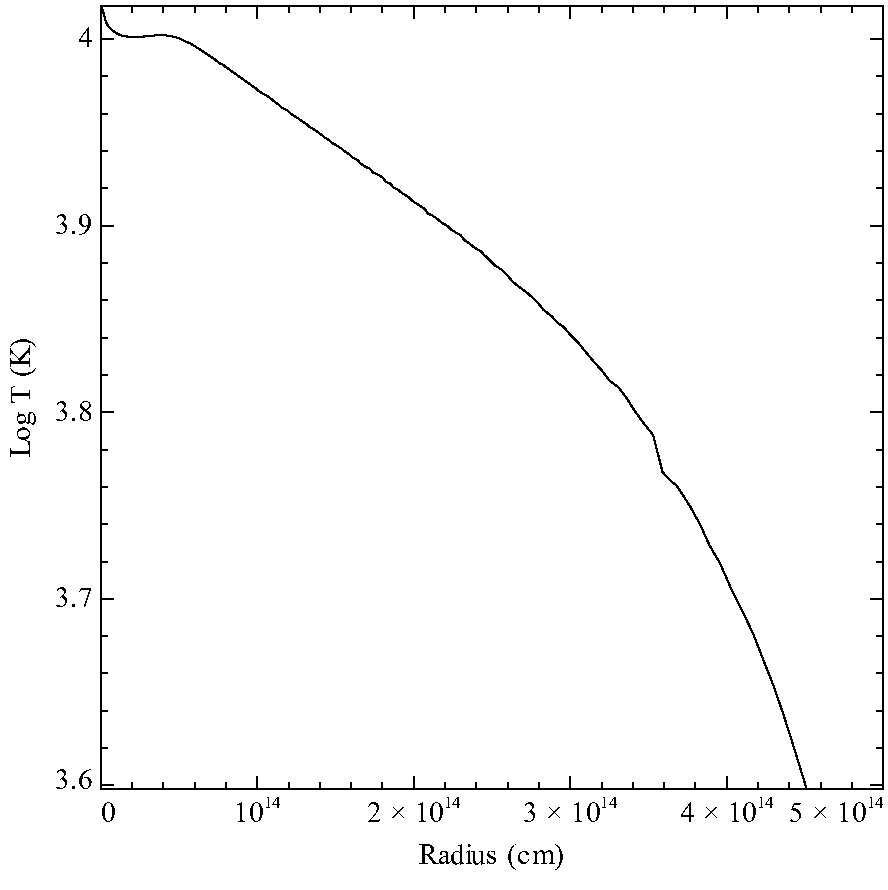
\includegraphics[clip=on,width=0.8\columnwidth,height=0.8\textheight,keepaspectratio]{PN_temperature}
\end{center}
\caption{The gas kinetic temperature as a function of radius for a simple planetary nebula.}
\label{fig:PN_temperature}
\end{figure}

\begin{figure}
\begin{center}
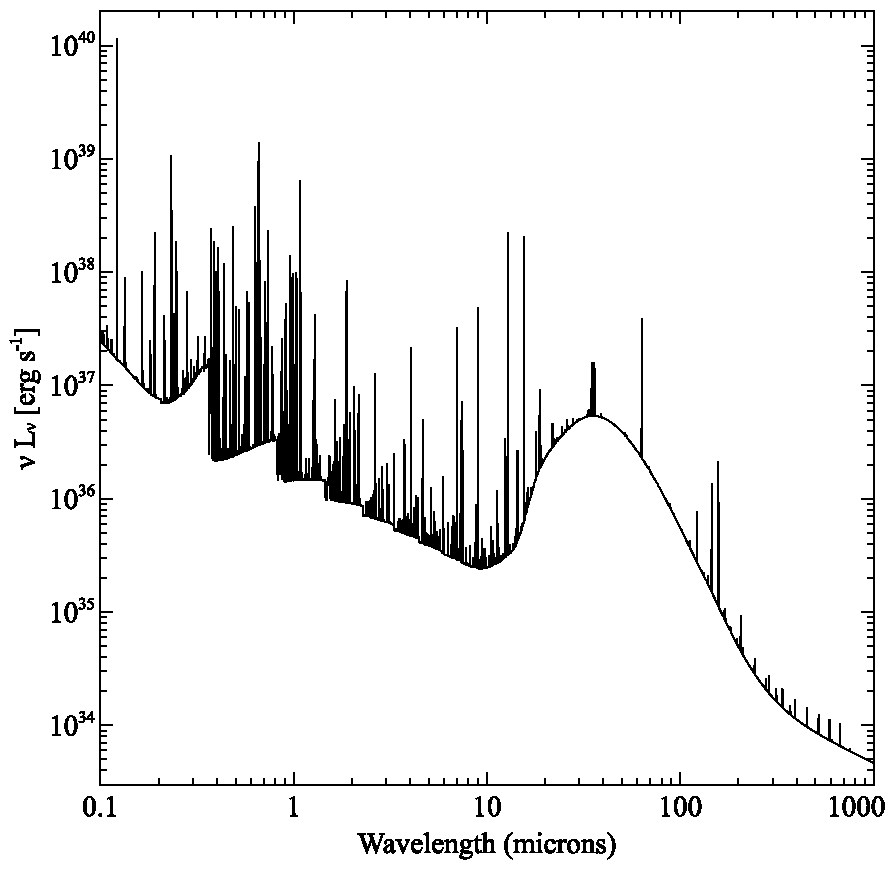
\includegraphics[clip=on,width=0.8\columnwidth,height=0.8\textheight,keepaspectratio]{PN_spectrum}
\end{center}
\caption{The spectrum of a planetary nebula.
The $x$-axis is the wavelength in microns.
The $y$-axis is $\nu L_\nu \rm{[erg\ s^{-1}]}$.
The large bump peaking at $\sim 30$\micron\ is
due to thermal dust emission.
Most of the emission lines are hydrogen and helium recombination lines
although strong forbidden lines are also present.
Several radiative recombination edges are present
across the optical -- IR spectral region.}
\label{fig:PN_spectrum}
\end{figure}

Dust in the nebula, warmed by light from the central star, produces the
large emission feature centered at $\sim 30$\micron\ (Chapter 7 of AGN3).
Recombination continua (Chapter 4 of AGN3) produce the cliff-like features
in the optical and near infrared.  The emission lines are produced by both
recombination (AGN3 Section 4) and collisional excitation (AGN3 Section
3).

\subsection{A quasar cloud}
\label{sec:QuasarCloud}

Next compute a simple model of a cloud in the quasar
broad emission-line region (BLR).
The BLR clouds are located close to the central engine of an active nucleus
(see Chapters 13 and 14 of AGN3) and they probe conditions near the most
massive structures that formed in the young universe.  The shape of a quasar
continuum is often fitted by a set of power laws.  Most of the literature
in this field describes the continuum intensity in terms of the flux of
photons in the hydrogen-ionizing continuum
$\varphi(\mathrm{H}) [ \pscm\ \ps ]$.
This is the intensity case described in
Section \ref{sec:LuminosityVsIntensityCases}
on page \pageref{sec:LuminosityVsIntensityCases}.
\small
\begin{verbatim}
table power law  # a built-in power-law continuum
phi(H) 18.5      # the log of the flux of H-ionizing photons [cm-2 s-1]
\end{verbatim}
\normalsize
A number of different spectral shapes are stored in the code as look-up
tables.  This \cdCommand{table} command uses
a power-law continuum with a slope $f_\nu \propto \nu^{-1}$
in the visible/UV and with a roll over in the X-rays and infrared.
The intensity of the incident radiation field is given as a flux of
photons that are capable of ionizing hydrogen [cm$^{-2}$ s$^{-1}$].
A starting radius does not need to be specified since this is
the intensity case.

We still need to specify a hydrogen density and a stopping
criterion\footnote{A planetary nebula is ionized by a hot star while the radiation
field striking a BLR cloud is very energetic, extending far into the $\gamma$-Rays.
The gas temperature falls to $\sim 100 \rm{K}$
on the neutral side of the $\mathrm{H}^+$--$\mathrm{H}^0$
ionization front in a PN since little radiation penetrates through the front.
In a BLR cloud a warm partially ionized zone, heated by X-Rays, extends
beyond the front so a stopping criterion must be specified.  This is one
of the major differences between a cloud ionized by starlight and one ionized
by a hard non-thermal continuum.}
A density of $\approx 10^{10} \rm{cm^{-3}}$ is
deduced from ratios of emission lines (AGN3
Chapter 13).
Most published calculations specify a total column density
to define the outer edge of the cloud.
Let's stop at a total hydrogen column density
of $10^{22}\ \pscm$.
This is large enough for an \hplus -- \hO\
ionization front to be present within the cloud.
Solar abundances are fine so we will not change these.
The covering factor, the fraction of $4\pi$ \sr\ covered by gas, is
small so the \cdCommand{sphere} command is not included.  We have:
\small
\begin{verbatim}
hden 10  # log of hydrogen density cm-3
stop column density 22  # log of hydrogen column density cm-2
\end{verbatim}
\normalsize
Many line transfer effects are very important in the BLR.  It is necessary
to iterate on the solution to converge the optical depths.  
But we only want to see the results from the last iteration.
We do this by
including the following commands
\small
\begin{verbatim}
iterate to convergence
print last iteration
\end{verbatim}
\normalsize
We will create the same two save files but with different file names
\small
\begin{verbatim}
save overview "blr.ovr" last
save continuum "blr.con" units microns last
\end{verbatim}
\normalsize
The keyword \cdCommand{last} says to save results
for the last iteration, 
similar to the command \cdCommand{print last iteration}.
The entire
input script, which we will call \cdFilename{blr.in}, is as follows.
\small
\begin{verbatim}
title BLR spectrum in Quick Start Guide
table power law  # a built-in power-law continuum
phi(H) 18.5      # the log of the flux of H-ionizing photons [cm-2 s-1]
#
hden 10          # log of hydrogen density cm-3
stop column density 22  # log of hydrogen column density cm-2
#
iterate to convergence
print last iteration
#
save overview "blr.ovr" last
save continuum "blr.con" units microns last
\end{verbatim}
\normalsize
The lines beginning with ``\#'' are comments and are ignored.
Run the code like we did before.
Examine the main output \cdFilename{blr.out} and make
the same plots of the temperature structure and emitted radiation field.
The predicted radiation field is shown in Figure \ref{fig:BLR_spectrum}.

\begin{figure}
\begin{center}
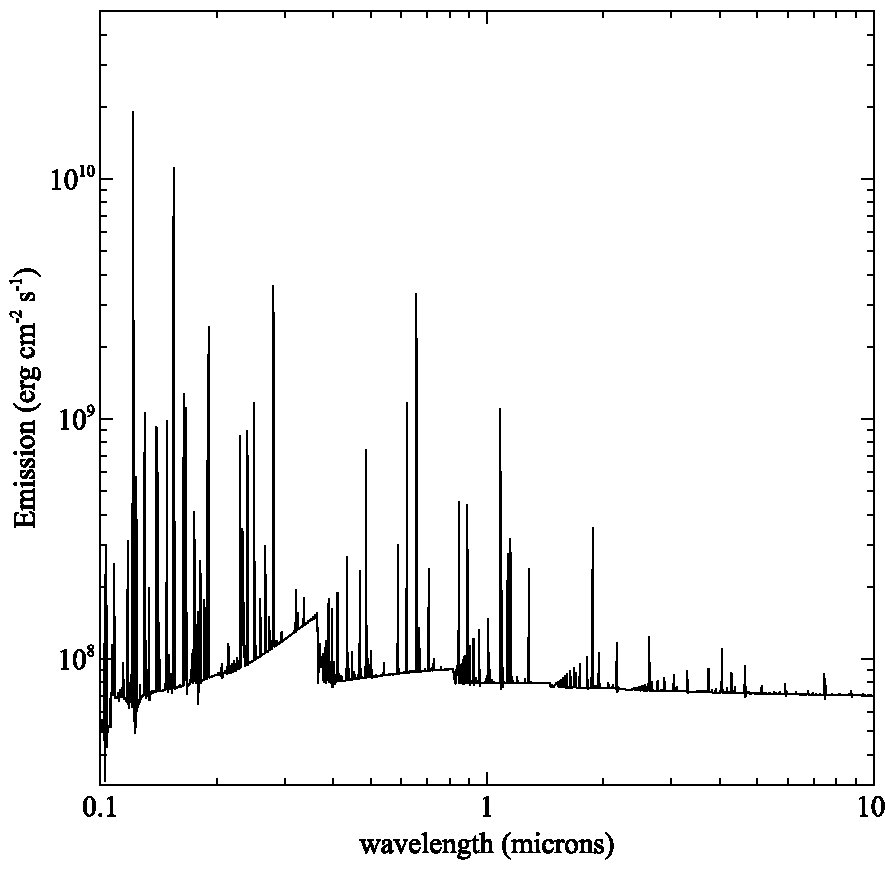
\includegraphics[clip=on,width=0.8\columnwidth,height=0.8\textheight,keepaspectratio]{BLR_spectrum}
\end{center}
\caption{The spectrum of a single broad emission-line
cloud in an active nucleus.
The $x$-axis is the wavelength in microns.
The $y$-axis is $\nu f_\nu [\erg\, \pscm\, \ps]$.}
\label{fig:BLR_spectrum}
\end{figure}

These are nearly the simplest models that can be calculated.  The
following sections go over each of the parameters described above and point
to sections of \Hazy\ that go into more detail.

\subsubsection{Heads up!}

Most commands expect numerical parameters
on the command line to be in
a particular order although they can often be omitted from right to left.
Be sure to follow the rules for each command.  Default values are assumed
when an optional parameter is missing.

Cloudy is designed to be autonomous and self aware.  It continuously
audits itself as a calculation progresses.  The end of the calculation may
have comments on various aspects of the
physics.
If problems occur then
the code may generate a warning or caution.
These are described further in Section~\ref{sec:WarningsCautionsSurprisesNotes}
on page \pageref{sec:WarningsCautionsSurprisesNotes}.

\section{Geometry}
\label{sec:Geometry}

\subsection{Zones and iterations}

The code works by dividing a cloud into a large number of thin layers
called zones.  There is a default limit of 1400 zones, but this can be
changed with the \cdCommand{set nend} command.
The code will generate a warning if
the calculation stops because the default limit to the number of zones was
reached since this probably was not intended.

By default the code will do one iteration, one complete simulation of
a cloud.  If line or continuum transfer is important then more than one
iteration will be necessary for a valid solution since the optical depths
must be known.  The number of iterations is controlled with the
\cdCommand{iterate}
command.  The code will complain if too few iterations were performed for
the optical depth scale to be converged.

\subsubsection{Commands normally used}

Frequently-used commands follow:

\cdCommand{set nend} changes the default limit to the number of zones.

\cdCommand{stop zone} tells the code to stop
at a particular zone.  This is mainly
used for debugging, or, in the case of \cdCommand{stop
zone 1}, to only compute the cloud's illuminated face.

\cdCommand{iterate} sets the number of iterations
to be performed.  The default is
a single iteration and more will be needed when radiative transfer effects
are important.  There is a special version of the command,
\cdCommand{iterate to convergence},
which tells the code to iterate until line and continuum optical
depths become stable.

\subsubsection{Heads up!}

The code will generate a warning
if it stops because it reaches the
default limit to the number of zones since this probably was not intended.
Use the \cdCommand{set nend} command to increase
the limit to the number of zones.

The code will generate warnings
or cautions if the optical depth scale
changes in the last iteration.
Increase the number of iterations if this
occurs with the \cdCommand{iterate} command
or use the \cdCommand{iterate to convergence} command.

\subsection{The geometry---intensity \& luminosity cases}

The brightness of the radiation field striking the cloud can be specified as
an intensity or luminosity.
It must be possible for the code to deduce the energy
striking a unit area of the cloud.
The subsection \emph{Intensity vs luminosity commands}
of Part~1 of \Hazy\ describes the
distinction between these two cases.

In the intensity case the energy flux (erg
cm$^{-2}$ s$^{-1}$) or photon flux (cm$^{-2}$
s$^{-1}$) striking a unit area of cloud is set.
The inner radius does not need
to be specified.
The emission per unit area
[erg cm$^{-2}$ s$^{-1}$] is predicted\footnote{The emission
per unit area is called the ``intensity'' in this
document, in the code, and in \Hazy.  For an optically thick slab this is
actually the emittance.  For an optically thin source this is $4\pi J$ where
$J$ is the mean intensity as defined in most radiative transfer texts.}.

In the luminosity case the total luminosity of the central source of
radiation is specified and the inner radius of the cloud must be set.  The
luminosities of emission lines [erg s$^{-1}$] are predicted.

The gas covering factor $\Omega/4\pi$
(AGN3 Section 5.9) is the fraction of $4\pi \sr$ covered by gas
as seen from the central object.  If the central object
has a total luminosity $L$ then the nebula
intercepts $L\Omega/4\pi$ of the radiation
field.  The covering factor will linearly affect line luminosities but have
only second-order effects on line intensities.

If the code can determine the separation [cm] between the continuum source
and the cloud then it will predict emission-line luminosities.  Otherwise
it will predict line intensities.  This is described further in the section
``Geometry'' of Part 1 of \Hazy.

\subsubsection{Commands normally used}

Frequently-used commands follow:

\cdCommand{radius} sets the inner radius
of the cloud.  Line luminosities can be
predicted if this is specified.  The command can also specify the cloud
thickness.

\cdCommand{covering factor} sets the covering factor of the cloud
$\Omega/4\pi$.  The
predicted emission-line luminosities scale linearly with the covering factor.

\subsubsection{Heads up!}

   None yet.

\subsection{Open or closed geometry}

   The chapter \cdTerm{Definitions} of Part~1 of \Hazy\ defines open and closed
geometries and the chapter \cdTerm{Geometry} goes into more details.  These
considerations affect the transfer of diffuse fields and only change the
predicted line intensities at the $\sim 10\%$ level.

   An open geometry is the default.  This is one where diffuse emission
from the illuminated face of the cloud escapes from the system without
striking other clouds.

   A closed geometry is one where gas covers most of the continuum source.
The \cdCommand{sphere} command sets this case.
Emission from the illuminated face of
the cloud passes the continuum source and strikes gas on the far side.

There are two classes of closed geometries, static and expanding.  In
the expanding case, the default when the \cdCommand{sphere} command is included,
line photons that cross the central cavity will not be absorbed
by gas on the far side due to Doppler shifts.  In the static case (the
\cdCommand{sphere static} command) emission lines
cross the central hole and are absorbed on
the far side.  These considerations have little effect on most lines but
do affect emissivity of higher-$n$ Lyman lines of hydrogen.

This is described further in the section in Part~1 of HAZY where the
\cdCommand{sphere} command is discussed.

\subsubsection{Commands normally used}

Frequently-used commands follow:

\cdCommand{sphere [expanding, static]}
\label{command:sphere}
tells the code to assume a closed geometry.
The shell can be either static or expanding.  By default the shell is assumed
to be expanding rapidly enough that lines escaping from the illuminated
face of the shell do not interact with the gas on the far side of the central
hole.  If the \cdCommand{static} keyword appears
on the \cdCommand{sphere} command then lines
escaping from one side will be absorbed by gas on the far side.  The
expanding option does not change the intrinsic line width, which is still
assumed to be thermal.  It only changes whether lines formed in opposite
sides of the shell interact.

\subsubsection{Heads up!}

These considerations affect the transport of the diffuse fields and have
only second-order effects on the predicted spectrum or physical conditions
in the gas.  If you are uncertain about the geometry, try the simulation
with and without the \cdCommand{sphere} command,
and try both \cdCommand{sphere static} and \cdCommand{sphere
expanding}.  Is this distinction important?  It usually is not.

\subsection{Is the gas static or a wind?  Is it turbulent?}

The cloud is normally assumed to be stationary.  Lines are broadened
only by thermal motions.  A component of microturbulence can be added and
a wind can be computed.

\subsubsection{Commands normally used}

Frequently-used commands follow:

\cdCommand{turbulence} adds a component of
microturbulence to line broadening.  This
will make line pumping by the incident radiation field more important and line
trapping less important, so it does affect the spectrum.  The parameter
is the turbulent velocity $u_\mathit{turb}$ in km s$^{-1}$.
\label{sec:TurbulenceWind}

The velocity entered in the \cdCommand{turbulence}
command is the component of
turbulence $u_\mathit{turb}$ that is added to the thermal width $u_\mathit{th}$
\begin{equation}
u = \sqrt {u_{th}^2  + u_{turb}^2 }\quad \rm{[\kmps]}
\end{equation}
to determine the total line width $u$.

\cdCommand{wind} simulates an expanding wind.
A static cloud is assumed by default.
The equations of motion determine the velocity as a function of depth.
LVG or Sobolev approximation escape probabilities are used for the line
transfer.  The parameter is the initial wind velocity in km s$^{-1}$.

The effects of both commands are discussed further in the sections in
Part~1 of \Hazy\ where these commands are described.

\subsubsection{Heads up!}

If turbulence is included then a turbulent pressure term is added to
the gas equation of state, the relationship between density and pressure.
This affects the density within constant-pressure clouds.  The gas equation
of state is discussed in the \emph{Optical Depths and Radiative Transfer}
chapter in Part~1 of \Hazy.

The velocity that appears on the \cdCommand{turbulence}
command is in km s$^{-1}$ because
observed velocities are always expressed in these units. Cloudy actually
works in cgs units.

The line width used in optical and UV astronomy is not the same as the
line width used in radio astronomy.
The description of the \cdCommand{turbulence} command in Part~1 of
\Hazy\ gives more information.

\subsection{What sets the outer edge to the cloud?
Why should the calculation stop?}
\label{sec:StoppingCriteria}

The code starts at the illuminated face of the cloud and works its way
into deeper regions.
This integration must stop for some reason.
In many
cases the outer edge of the simulation is not the outer edge of the cloud
but rather the region where the gas has become cold and neutral.  In other
cases the column density of the cloud may be known from observations.  Many
different stopping criteria can be specified and the code will stop when
the first one is reached.

Cloudy was originally designed to interpret optical/UV emission lines
in quasars.  These lines are produced in warm ionized gas so the default
is to stop the calculation when the gas temperature falls below 4000~K.
This will often be near the hydrogen ionization front.  This would be a
mistake if you want to consider cool atomic or molecular regions.

You should understand what sets the outer edge of the cloud you wish
to simulate and then confirm that the code reached that point.  The
introduction to the chapter \emph{Stopping Criteria}
of Part~1 of \Hazy\ goes into
this in more detail.

\subsubsection{Commands normally used}

Frequently-used commands follow.
These are only a small fraction of the many ways that
a calculation can be stopped.

\cdCommand{radius} sets the inner and outer radius of the cloud.

\cdCommand{stop temperature} sets the lowest
kinetic temperature to allow.  The
calculation will stop when the temperature falls below this value.  The
default is 4000~K.  This will usually cause the calculation to stop near
the H$^+$--H$^0$ ionization front.  You must
set a lower temperature if you want
the calculation to extend into the PDR or molecular cloud.

\cdCommand{stop thickness} sets the thickness
of the cloud, the distance from the
illuminated face to the shielded face, the outer edge of the cloud.

\cdCommand{stop column density}  sets an upper
limit to the hydrogen column density
[cm$^{-2}$].
The default is to include hydrogen in all forms (H$^0$,
H$^+$, and H$_2$) in this column density
although keywords can be used to select only species
like \hplus\ or \hO.

\cdCommand{stop efrac} stops the calculation
when the electron fraction, $n_e/n(\mathrm{H})$,
falls below the specified value.  This makes it easy to stop near ionization
fronts.

\cdCommand{stop Av} stops the calculation at a
certain visual extinction.
By default the $A_V$ will be for a point source,
which is the quantity measured in extinction studies of stars.
The extended-source extinction, appropriate for extinction
across a cloud, is specified with the keyword \cdCommand{extended}.

\cdCommand{double}
\label{command:double}
This doubles the computed optical depths at the end of an
iteration.  This command should be used if the region being simulated is
only a layer on a much larger structure.  This is the case in a PDR
calculation, where an unmodeled molecular cloud is assumed to lie beyond
the shielded face of the PDR.  Lines will be quite optically thick at this
outer edge.  Emission from the shielded face will be suppressed if this
command is used since we then assume that the layer is the mid plane of
the cloud. Were this command not included the code would assume that the
outer edge of the model is the outer edge of the cloud and optically thick
lines would freely radiate from the shielded face.  This is unphysical.
The physics is described further in the chapter
\emph{Optical Depths and Radiative Transfer} of Part~1 of \Hazy.

\subsubsection{Heads up!}

The \cdCommand{stop temperature} and \cdCommand{stop efrac}
commands are useful ways to stop
a calculation in the PDR or molecular cloud.
Use the \cdCommand{stop temperature}
command by itself to stop the calculation at a low temperature.
Set the stopping temperature to a very low value
and use the \cdCommand{stop efrac} command
to stop the calculation when the electron fraction falls below a certain
value.

The calculation will stop when it reaches a depth where any of the
stopping criteria are satisfied.
Understand why the calculation stopped.
Did it stop for the reason you expected or did it stop prematurely because
another criterion was met or because the calculation had problems?  Is the
calculation a complete simulation of the region you want?  The code will
explain why it stopped in the first lines after the last zone.
A sample printout of the last zone and the explanation for why the calculation stopped follows.

\label{sec:ZoneOutput}
{\setverbatimfontsize{\tiny}
\begin{verbatim}
####259  Te:2.980E+01 Hden:1.000E+05 Ne:2.441E-01 R:1.000E+30 R-R0:1.408E+17 dR:7.588E+15 NTR: 27 Htot:9.894E-24 T912: 9.14e+04###
 Hydrogen      6.68e-01 2.44e-06 H+o/Hden 6.68e-01 6.63e-14 H-    H2 1.66e-01 7.65e-14 H2+ HeH+ 8.86e-15 Ho+ ColD 9.92e+21 1.01e+17
 Helium        1.00e+00 5.20e-08 0.00e+00 He I2SP3 1.14e-15 Comp H,C 1.78e-30 5.98e-31 Fill Fac 1.00e+00 Gam1/tot 1.58e-02
 He singlet n  1.00e+00 5.81e-22 9.19e-27 8.61e-29 4.08e-28 3.12e-28 He tripl 1.14e-15 1.12e-26 1.53e-28 1.66e-27 8.53e-28
 Pressure      NgasTgas 2.70e+06 P(total) 3.73e-10 P( gas ) 3.73e-10 P(Radtn) 2.14e-17 Rad accl 3.99e-14 ForceMul 8.66e+00
               Texc(La) 2.95e+03 T(contn) 3.00e+01 T(diffs) 6.30e-01 nT (c+d) 7.39e+06 Prad/Gas 5.75e-08 Pmag/Gas 0.00e+00
 Lithium       2.20e-01 7.80e-01 0.00e+00 0.00e+00 Berylliu 6.14e-01 3.86e-01 0.00e+00 0.00e+00 0.00e+00 sec ion: 1.34e-17
 Carbon        0.00e+00 0.00e+00 0.00e+00 0.00e+00 0.00e+00 0.00e+00 0.00e+00 H2O+/O   0.00e+00 OH+/Otot 0.00e+00 Hex(tot) 0.00e+00
 Nitrogen      0.00e+00 0.00e+00 0.00e+00 0.00e+00 0.00e+00 0.00e+00 0.00e+00 0.00e+00 O2/Ototl 0.00e+00 O2+/Otot 0.00e+00
    model of cloud with primordial abundances exposed to background at Z=10
   Calculation stopped because lowest Te reached.    Iteration 2 of 2
   The geometry is plane-parallel.
\end{verbatim}
}

\subsection{What about clumping?}

Clumping can be included.  There are three general considerations.

There are powerful selection effects at work when a range of densities
exist.  You will tend to observe the highest-density regions because the
emission per atom is proportional to density if the line is below its
critical density (see AGN3 Section 3.5 and
Figure \ref{fig:CIV_equivalent_width}
on page \pageref{fig:CIV_equivalent_width}).
Only with a particular mix of
densities, where the amount of material at each density exactly compensates
for the change in emissivity, will an observer notice emission from a range
of densities.  So I am always very skeptical of claims that a range of
densities contribute to a single emission line.
This would require an amazing coincidence 
\citep{Ferland.G11Molecular-hydrogen-in-NLSys-and-its-implications}.

But clumps do exist.
If the clump size is small compared with the
physical thickness of the H$^+$ region then they can be treated with a filling
factor (see the discussion in
Section~\ref{command:FillingFactor} on page
\pageref{command:FillingFactor},
 AGN3 Section 5.9, and \citet{Osterbrock1959}).
In this
case the gas is modeled as small clumps that are surrounded by vacuum or
much lower-density gas.
This is done by simply including the
\cdCommand{filling factor} command to specify the fraction
of the volume that is filled by clumps.

If the clumps are larger than the physical thickness of the H$^+$ region
then each clump will have its own ionization structure.
This is the ``LOC''
model of quasar emission-line clouds described by
\citet{BaldwinEtAl95}.
The model is developed in several papers by the same team.
In this case
we compute grids of models and save the results.  The spectra are then
co-added using distribution functions to describe the range of cloud
properties.  The final spectrum depends on these distribution functions.
The program \cdFilename{mpi.cpp} in the programs directory in the code distribution
computes a grid of models and extracts the predictions using MPI to parallelize
the computations.
The \cdCommand{grid} command (see
Section~\ref{sec:GridsOfModels} on page
\pageref{sec:GridsOfModels}) can also
be used to compute large numbers of models.
\citet{GiammancoEtAl_clumpsCloudy04} show \Cloudy\ calculations
where optically thick clumps are present in the ISM.

Complex geometries are done by using \Cloudy\ to compute volume elements
within a much larger cloud.
An example is the Cloudy\_3D code,
available from 
\href{http://sites.google.com/site/cloudy3d/}{sites.google.com/site/cloudy3d}
and described in \citet{MorissetCloudy3D06}
and \citet{MorissetStasinskaCloudy3D08}.
An image is shown in \Hazy\ 1.
The RAINY3D code is another example 
\citep{MoraesDiazRAINY09}.


\section{Composition and density}
\label{sec:CompositionAndDensity}

What is the chemical composition of the gas?
Should grains be included?
Should PAHs also be included?
Commands that set the composition are discussed
in the chapter \emph{Chemical Composition} of Part~1 of \Hazy.
The default
composition is close to solar and grains are not included.

The density at the illuminated face of the cloud, and a description of
how this density varies with depth, must also be given.
By default the
code will assume that the density and composition do not change across the
cloud.

\subsection{Chemical composition}

The composition is set by specifying the abundances of the lightest
30 elements.
Abundances are specified by number relative to hydrogen.
On this scale a typical carbon abundance is
$n(\rm{C}) / n(\rm{H}) \approx 2\times 10^{-4}$.

\subsubsection{Commands normally used}

Frequently-used commands follow:

\cdCommand{abundances} sets the abundances
\label{command:abundances}
of all elements to the values given on
the line.  If no numbers are present but a keyword is given then the
composition is set to a standard mixture.  Examples include the local ISM
or a typical planetary nebula.  Grains are included in some abundances sets.
Consult the \cdTerm{Chemical Composition} chapter
of Part~1 of \Hazy\ to find out more.

\cdCommand{element} sets the abundance of
\label{command:element}
a particular element, removes the element
from the calculation, or specifies its ionization state.

\cdCommand{grains} determines the type
\label{command:grains}
and abundance of grains.  If grains are
included then, by default, their abundance will be the same across the cloud
and quantum heating will be included when it is important.   The
\cdCommand{function}
keyword will make the grain abundance depend on position and the
\cdCommand{no qheat}
keyword will turn off quantum heating.  By itself this command specifies
classical or large grains but does not include PAHs.

\cdCommand{grains PAH} includes PAHs.  By default
their abundance will be proportional
to the ratio $n(\mathrm{H}^0)/n(\mathrm{H}_\mathrm{tot})$
as suggested by observations of the Orion Bar (Section 8.5 of AGN3).

It is easy to create new types of grains by specifying their refractive index
and size distribution data.
This is described in the appendix \emph{Using the Grain Code in Cloudy} in Part~1 of \Hazy.

\cdCommand{metals} changes the abundances
\label{command:metals}
of the ``metals'' (all elements heavier
than helium) by the scale factor given on the command line.  It can also
change the gas to dust ratio or set depletion factors for the gas-phase
abundances of the elements.

\subsubsection{Heads up!}

\emph{Grain sublimation:} A warning will be printed if grains become hotter
than their sublimation temperature.  They will not be removed from the
calculation.  The effects of grain sublimation can be mimicked by making
the grain abundance vary with depth with the
\cdCommand{function} option on the \cdCommand{grains}
command but this requires writing a new routine.  Note also that if grains
are destroyed the material contained within them must be returned to the
gas phase to be self consistent.  This also is not done automatically.
Finally, a note will be printed if grains are not present but could exist
since they would have been below their sublimation temperature.

\emph{Gas-phase abundances and grains:}
It is possible to leave the gas-phase
composition at its solar value, appropriate if all elements are in the gas
phase, but also set a population of grains
with the \cdCommand{grains} command.  This
is not consistent.  When grains are present the elements that comprise them
are depleted from the gas phase.  If you use solar gas-phase abundances
and assume that grains exist then the code will complain but still perform
the calculation.

\emph{PAH abundances:} There is good observational
evidence that PAHs only exist
in the H$^0$ region (AGN3 Section 8.5).  Observations of the Orion Bar suggest
that they are destroyed in the H$^+$ region and coagulate into larger grains
in molecular regions.  By default the PAH abundance depends on the ratio
$n(\mathrm{H}^0)/n(\mathrm{H}_\mathrm{tot})$.  Other
dependencies on depth can be used by changing the
routine called when the function keyword is used.

\subsection{What is the cloud's density?  Does it vary with depth?}

The density of hydrogen is used to set the cloud density.  The default
is for the hydrogen density to be the constant value set by the
\cdCommand{hden} command.
Optional commands tell the code to assume constant pressure, include a
magnetic field or turbulence in the pressure, or to vary the density with
a function specified by the user.  Most of these are discussed in chapter
\emph{Density Laws} of Part~1 of \Hazy.

\subsection{Commands normally used}

Frequently-used commands follow:

\cdCommand{hden} specifies the log of the
\label{command:hden}
hydrogen density [cm$^{-3}$].  Constant density
is the default.  This includes hydrogen in all forms.

\cdCommand{constant pressure}\quad The cloud will be isobaric or
\label{command:ConstantPressure}
in hydrostatic equilibrium.  The equation
of state includes pressure terms from thermal gas motions, turbulent motions,
a magnetic field, the nearly isotropic radiation pressure produced by trapped
emission lines, and the outward push of the incident radiation field on
the gas.  The keyword \cdCommand{gas} says to
keep the gas pressure, rather than the
total pressure, constant.
This is discussed in the
\emph{Optical Depths and Radiative Transfer} chapter in Part~1 of \Hazy.
Self-gravity of the gas can be included with the \cdCommand{gravity} command, described in chapter \emph{Density Laws}.

\cdCommand{filling factor}\quad  The gas is
\label{command:FillingFactor}
normally assumed to fully fill the available
space.  This command sets a filling factor $f,$ the fraction of the volume
that contains gas (AGN3 Section 5.9).  The remainder of the volume is a
vacuum.

\cdCommand{magnetic field}\quad These are ignored
\label{command:MagneticField}
by default.  Magnetic fields will
contribute to the total pressure, and, optionally, to the turbulent velocity
field.  The parameters specify the magnetic field at the illuminated face
and the field geometry.
Cyclotron cooling may become important if the
temperature is high enough.
All of this is discussed in the chapter
\cdTerm{Thermal Solutions} of Part 1 of \Hazy.
The gas and field are assumed to be well
coupled so the magnetic pressure terms are included in constant pressure
models.

\subsubsection{Heads up!}
\cdCommand{hden} gives the \cdTerm{total hydrogen density}, defined as
\begin{equation}
n\left( {\rm{H}} \right) = n\left( {{\rm{H}}^{\rm{0}} } \right) + n\left(
{{\rm{H}}^ +  } \right) + 2n\left( {{\rm{H}}_2 } \right) +
\sum\limits_{other} {n\left( {{\rm{H}}_{other}^{} } \right)}
\quad \rm{[cm^{-3}]}
\end{equation}
where the sum includes H in other molecules and H$^-$.  In nearly all cases
hydrogen will be in one of the first three forms.

Turbulent and magnetic pressure, as well as gravity, can be included in the total pressure
of a \cdCommand{constant pressure} cloud.

\section{The incident radiation field}
\label{sec:IncidentRadiationField}

Often the radiation field striking the cloud is its only energy source.
The radiation field is specified by its shape, which describes how it depends
on wavelength or frequency, and by its intensity or luminosity.  The shape
and intensity are usually specified with different commands.
The chapter
\emph{Defining the Continuum} of Part 1 of
\Hazy\ gives an overview of how this is
done.  More than one continuum source can be included.  The following
sections describe how to specify both the shape and intensity.

\subsection{Luminosity vs intensity cases}
\label{sec:LuminosityVsIntensityCases}

In general the radiation field striking the cloud can be specified either
of two ways.
In the \cdTerm{luminosity case}
the total luminosity emitted by the
central object and the inner radius of the
cloud are given.
In the \cdTerm{intensity case} only the flux of radiation striking
the cloud is specified.

\subsection{The luminosity or intensity of the incident radiation field}

There are many ways to specify the intensity or luminosity.
These are described
in the chapter \cdTerm{Continuum Luminosity} of Part~1 of \Hazy.
By default most
luminosity or intensity commands specify the quantity integrated over
hydrogen-ionizing energies.  Most also have
the \cdCommand{range} option, which allows
this energy range to be changed.

\subsubsection{Commands normally used}

Frequently-used commands follow:

\cdCommand{Q(H)} specifies the number of
hydrogen-ionizing photons emitted by the
central object into $4\pi\,\rm{sr} \rm{[s^{-1}]}$ (AGN3 Section 2.1).

\cdCommand{phi(H)} is the intensity
[$\rm{cm^{-2}\, s^{-1}}$] equivalent of the \cdCommand{Q(H)} command.
It sets $\phi(\mathrm{H})$,
the flux of hydrogen-ionizing photons striking the face of the cloud.

\cdCommand{luminosity} specifies the luminosity
emitted by the central object into
$4\pi \sr\ [\ergps ]$.  By default this
is the luminosity in H$^0$-ionizing radiation.

\cdCommand{intensity} is the intensity
$[\rm{erg} \ \rm{cm}^{-2} \ \rm{s}^{-1}]$
equivalent of the \cdCommand{luminosity}
command.  It gives the intensity of radiation striking the cloud face.
Note that this ``intensity'' is $4\pi$ times
larger than the true mean intensity
$J,$ which has units $\rm{erg\, cm^{-2}\, s^{-1}\, sr^{-1}}$.

\cdCommand{ionization parameter}\quad  This
sets the dimensionless ratio of densities
of ionizing photons to hydrogen, $U\equiv
\phi(\mathrm{H})/cn(\mathrm{H}_\mathit{tot})$
(AGN3, equation 14.7, page 357).  The number is the log of $U$.  This
can sometimes be useful since clouds with the same ionization parameter
have similar levels of ionization and temperature.  This is equivalent to
an \cdCommand{intensity} command.

\subsubsection{Heads up!}

None yet.

\subsection{The shape of the incident radiation field}

The continuum shape can be interpolated from a table of points, specified
as a fundamental form such as a blackbody or bremsstrahlung, or taken from
a previous Cloudy calculation.  Methods of setting the shape are described
in the chapter \emph{Continuum Shape} of Part~1 of \Hazy.

The shape should be specified between the code's limits of \emmmhz\
(the lowest frequency observable with LOFAR)
and \egamrymev, if possible.  The code will complain but compute
the model if the continuum is not specified over the full energy range.

The absolute values of the numbers giving the shape do not matter.  The
shape is renormalized to have the intensity set with an intensity command.

\subsubsection{Commands normally used}

Frequently-used commands follow:

\cdCommand{table SED} will interpolate on a table giving
pairs of frequency/intensity points.  This is the most commonly used method
of setting the shape since the results of other calculations,
such a stellar atmosphere, can be directly entered.

\cdCommand{table STARS} is an expanded form of the \cdCommand{table SED} command
which makes it possible to interpolate upon grids of SEDs predicted by stellar atmosphere models.
The command has its own subsection in \Hazy\ 1 and is further described on the \emph{Stellar atmospheres}
section of the \emph{nublado.org} web site.

\cdCommand{interpolate} is an older method of specifying
the SED as a table of points.

\cdCommand{CMB} adds the cosmic microwave background for any redshift.

\cdCommand{blackbody} specifies a blackbody.
This command has a number of options
that allow the intensity of the radiation field to be specified using
blackbody relationships.

\cdCommand{background} is a simple estimate
of the X-ray/UV background at any
redshift.  It includes the CMB.

\cdCommand{table [keyword]} gives one of a set of built-in
continua.  Some examples include
the AGN\slash starburst cosmic background at any redshift $z$, some stellar
continua, and the local ISM galactic background.

The \cdCommand{save transmitted continuum, table read} pair of commands
first saves the continuum transmitted through a first cloud, then uses the
\cdCommand{save transmitted continuum} command to include that
as part of the SED in a second calculation.  Examples of doing this
are the simulations 
\cdFilename{func\_trans\_save.in}, \cdFilename{func\_trans\_read.in},
\cdFilename{func\_trans\_read\_scale.in} in the test suite.  

\cdCommand{table AGN} enters the Mathews \& Ferland (1987) quasar continuum.

\cdCommand{table HM96} employs the Haardt
\& Madau (1996) background at a range of redshifts.

\cdCommand{table ISM} is the local ISM background.

\cdCommand{extinguish} \label{command:extinguish}will extinguish
the incident continuum by photoelectric
absorption due to a column density of neutral hydrogen.  This command is
often used to remove hydrogen-ionizing radiation in a PDR calculation.
The culture in this field is to assume that an unmodeled H$^+$ region has extinguished much of the incident radiation field.

\cdCommand{cosmic ray background} will include
galactic background cosmic rays.
These are important when the calculation extends into molecular gas.  The
chemistry of the cold ISM is driven by a series of ion-molecule reactions
that are initiated by cosmic-ray ionization.  The required ions will not
exist if no source of ionization is present and the chemistry network may
collapse.  The code will complain, but try to compute the model, if the
calculation extends into cool regions without including background cosmic
rays.

\subsubsection{Heads up!}

Some shape commands also specify
an intensity.  An example is \cdCommand{table HM96}, which
specifies both the shape and intensity of the quasar
background at some redshift. Commands that set both are listed in subsection
\emph{Keeping shape and intensity commands together}
of Part~1 of \Hazy, which also
describes a \emph{possible disaster.}

The shape of the incident radiation field
should be specified over the entire
energy range considered by the code, \emm\ to \egamrymev.   An easy way to do
this is to include, as a minimum, the cosmic microwave background and local
ISM diffuse continuum.

The incident radiation field is assumed to be completely reflected for frequencies
smaller than the plasma frequency of the cloud.  This often occurs for
moderate densities due to the very low frequencies that are included in
the continuum.

The chemistry convergence will struggle, and likely find bizarre results,
if the simulation extends into cold molecular regions but does not include
the cosmic ray background.  Interstellar chemistry requires a source
of ionization to drive the network.  
Include the \cdCommand{cosmic rays background} command
extends into the H$^0$ or \htwo\ regions.

The cosmic microwave background
should always be included with the \cdCommand{CMB}
command.  This is not done by default.
The command \cdCommand{no isotropic continua report}
may be used to {\em not} include the CMB (and any other
isotropic radiation fields) in the output fluxes.
This affects {\em only} the output -- \Cloudy\ always
includes them in the solution of the physics problem.

\cdCommand{table ISM} and \cdCommand{cosmic rays
background} should probably be included for
objects within our galaxy.

The quasar background continuum
should probably also be included using
either the \cdCommand{background} or \cdCommand{table HM} commands.

Pairs of intensity and shape commands should be kept together.  They
may be misinterpreted if they are not.

\section{Other commands}
\label{sec:OtherCommands}

\subsection{Radiative transfer}

All line-formation processes, including line trapping, collisional
deexcitation, continuum pumping, and destruction by background opacities
(see AGN3 Section 14.5), are included.

\subsubsection{Commands normally used}

Frequently-used commands follow:

\cdCommand{Case B} \label{command:CaseB}
artificially sets the
optical depths of hydrogen Lyman lines to
very large values.  Under some circumstances this will force the hydrogen
recombination lines to their Case B intensities, the limit where all Lyman
lines scatter often enough to be degraded into \la\ and
Balmer lines (AGN3, Section 4.2).
This command is only intended for setting up ``homework'' problems or test
cases and should never be used in a simulation of a real object.  It can
have unexpected effects.  If the cloud does not contain dust then the mean
intensity of $\mathrm{L}\alpha$ will become very
large when this is used.  This may result
in unphysical photoionization rates for
valence shells of third or fourth-row elements.

\cdCommand{Database H-like Lyman pumping off}   This command must be included in 
homework-problem PDRs in which the
H$^+$ region is ignored.  If the command were not included then a thin layer
of ionized gas would be produced on the face of the PDR.  This is produced
by photoexcitation of \hO\ by the continuum in the Lyman lines, followed by
decay into the metastable $2s$ \hO\ level, which is then photoionized by the Balmer
continuum.

\cdCommand{turbulence} and \cdCommand{wind}\quad  These
commands are discussed in section~\ref{sec:TurbulenceWind}
on page \pageref{sec:TurbulenceWind}.
They strongly affect line transfer by changing the line width and resulting
opacities.  The code assumes that only thermal motions broaden lines unless
an additional component of motion is added with one of these commands.

\subsubsection{Heads up!}

The \cdCommand{Case B} command has many
artificial side-effects, especially when
grains are not present.
It should not be used except in special test cases.

\subsection{The H$_2$ model}

A large and complete model of H$_2$ emission can be included.
It is slow and not used by default.  Very simple approximations
are used when the complete model is not included.  These
simple approximations may or may not be good representations of the physics
of the real molecule.

The large H$_2$ models is used when the \cdCommand{database H2}
command is included (see the chapter \emph{Optical Depths and Radiative Transfer}
of Part~1 of \Hazy).  There are also special save output options that allow
the emission or absorption from this complex species to be saved and analyzed.

The large model of H$_2$ was part of Gargi Shaw's thesis and is described
in \citet{Shaw2005}.
AGN3 describes some properties of H$_2$ in Section
8.3 and appendix A6.  The simulations \cdFilename{h2*.in}
in the test suites give examples
of its use.  The \cdCommand{save H2} command
gives a number of convenient output options.

\subsection{The optimize command}

The \cdCommand{optimize} commands make it
possible to solve the ``inverse problem,''
probably the most common research area in astrophysics.  This is when the
outcome, perhaps an observed spectrum, is known and we wish to derive the
conditions that created it.  We know the ``answer'' and wish to find the
``question.''

A set of observed quantities are specified in the input stream along with
a series of \cdCommand{optimize} commands.  The
keyword \cdCommand{vary} says which parameters should
be varied to try to reproduce the observed quantities.  The code will then
run a series of calculations, change the input parameters that include the
\cdCommand{vary} option, and try to find parameters
that match observations.
All of
this is described in the chapter \emph{The Optimize Command} of Part~1 of \Hazy.
The simulations \cdFilename{optimize*.in} in the
test suites show examples of its use.

It is generally a bad idea to write a paper that simply gives the result
of an optimized model.  This appears as a computational miracle with little
pedagogical value.  A better approach is to find the best-fitting parameters
then show a series of calculations in which various parameters are changed
around the best values.  Changes in predicted quantities can then be shown.
A discussion of physical cause of these changes will then motivate the final
``best'' model.

\subsection{Grids of models}
\label{sec:GridsOfModels}

The greatest physical insight is often obtained from looking at results
of grids of calculations to discover physical trends or correlations.  An
example is shown in Figure \ref{fig:CIV_equivalent_width}
giving the equivalent width of one of the
strongest emission lines in quasars as a function of two cloud parameters
(Hamann \& Ferland 1999).

\begin{figure}
\begin{center}
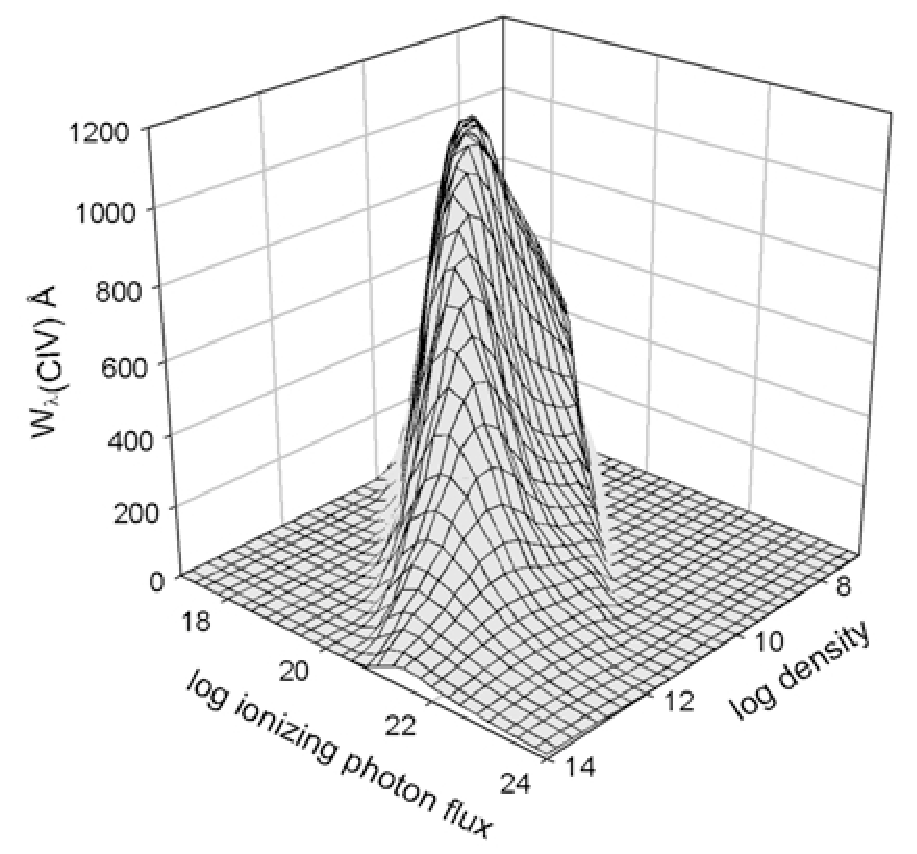
\includegraphics[clip=on,width=0.8\columnwidth,height=0.8\textheight,keepaspectratio]{CIV_equivalent_width}
\end{center}
\caption{The predicted equivalent width of
C IV $\lambda$1549\AA\ as a function of cloud density
and the flux of ionizing photons striking the cloud.  See Hamann \& Ferland
(1999) and Ferland (2003) for further details.}
\label{fig:CIV_equivalent_width}
\end{figure}

The code is designed to be used as a sub-program of other, larger, codes.
The command format is the same when it is used as a subprogram but commands
are entered by calling a special routine that contains the command line
as an argument.  Cloudy is then executed and the predictions are retrieved
after the simulation finishes.  This method of running the code is described
in the chapter \emph{Cloudy as a Subroutine} in Part~2 of \Hazy.
The test suite
directory includes a subdirectory \cdFilename{programs}
that includes a set of sample
programs that illustrate this use of the code.

The \cdCommand{grid} command, introduced by
Ryan Porter in C07, see \citet{PorterEtAl06},
makes it easy to do such a calculation without writing new code.  The
predictions in Figure \ref{fig:CIV_equivalent_width}
can be produced by modifying the simple BLR script
given in Section \ref{sec:QuasarCloud} on page
\pageref{sec:QuasarCloud} to read as follows:
\small
\begin{verbatim}
table power law
phi(H) 18.5 vary
grid from 17 to 24 in 0.5 dex steps
hden 10 vary
grid from 7 to 14 in 0.5 dex steps
stop column density 22
save line list "blr.line" no clobber "LineList.dat"
save grid "blr.grd" no clobber
\end{verbatim}
\normalsize

The \cdCommand{vary} keyword tells the code
which parameters to vary.  The \cdCommand{grid}
commands specify the lower and upper limits to the ranges over which the
previous parameter is to be varied and also give the step sizes.  The
parameters are varied by adding the step size to the initial value until
it exceeds the final value.  By default the grid is equally spaced in log space since
the values on the \cdCommand{grid} command are
logs.  The actual value of the parameter
given on the command with the \cdCommand{vary}
option is not used but must be present to satisfy the command parser.

There are several output options that are designed for use
with the \cdCommand{grid} command.
The \cdCommand{no clobber} option tells the \cdCommand{save}
command to write the output from each
model into the same save file rather than overwriting the file (clobbering
it) with each new simulation in the grid.

The \cdCommand{save line list} command makes
it possible to read in a list of lines
from the file given in the second pair of quotes and save the predicted
intensity into the first file.
This is how the results shown in Figure \ref{fig:CIV_equivalent_width}
were produced.
The labels in the file must include both the four character
string that is used in the output and the line wavelength.  They must match
exactly for the line to be recognized.

The \cdCommand{grid} command is described
in the chapter \emph{Miscellaneous commands} in
Part~1 of \Hazy\ and the \cdCommand{save line
list} command is described in the chapter
\emph{Controlling output} of Part~1.

\subsection{Miscellaneous commands}

\subsubsection{Commands normally used}

Frequently-used commands follow:

\cdCommand{atom} changes the treatment of
some model atoms.  It has many keywords.
\cdCommand{atom H-like} and \cdCommand{atom He-like}
allow some aspects of the H-like and He-like
isoelectronic sequences to be changed.  \cdCommand{H2}
turns on a large (and slow) model of \htwo\ \citep{Shaw2005} emission.

\cdCommand{init} Frequently-used commands
can be stored in one or more initialization file(s).
The \cdCommand{init} command will include the
contents of this file in the input stream.
The file name appears on the command line within a pair of double quotes.

\cdCommand{Comments} These can be included
within the input stream.
The section \emph{Introduction to Commands} of Part~1
of \Hazy\ explains how to enter several types of comments.
Generally, any line that begins with a sharp sign, ``\#'',
is taken as a comment and ignored.

\cdCommand{coronal time init}
This command can be used to study how a parcel of gas cools
under conditions of constant density (isochoric) or pressure
(isobaric).

\section{The code's predictions}
\label{sec:TheCodesPredictions}

\subsection{The default printout}

When the code is executed on a command line, as in
\small
\begin{verbatim}
cloudy.exe < test.in > test.out
\end{verbatim}
\normalsize
the file \cdFilename{test.in} contains the code's
input commands (read from \cdFilename{stdin}) and
its output (written to \cdFilename{stdout}) goes
to \cdFilename{test.out}.
The output is fully
described in the chapter \emph{Output} of Part~2 of \Hazy.
The default output
includes a copy of the input commands, a list of the abundances of the
chemical elements and grains, the physical conditions in the first and last
zone, an explanation why the calculation stopped, the intensity or luminosity
of the stronger emission lines, and the mean ionization, temperature, and
column density of many species.

\subsubsection{Commands normally used}

Frequently-used commands follow:

\cdCommand{title} enters a title that is printed at various places.

\cdCommand{print} commands change some aspects
of the printout.  It can sort the
emission lines, change their format, and modify what information is printed.

\cdCommand{print line faint xx}  The
predicted intensities of many lines are given
in the main printout.  Only the brighter lines are predicted since the total
number of lines is vast.  This command changes the limit to the faintest
line to print.

\cdCommand{normalize} The log of the radiated
luminosity or intensity of each emission
line is printed after the line's label in the main printout.
The intensity
of each line relative to a normalization line is also given.
In optical
emission-line spectroscopy the normalization line is usually
$\mathrm{H}\beta$ and this is the code's default.
The \cdCommand{normalize} command specifies
another line to use.

\subsection{Understand why the calculation stopped}

The reason the calculation stopped is given in the first
comments after the last zone and is described further in the introduction
to the chapter \emph{Stopping Criteria} of Part~1 of \Hazy.
An example of the last
zone printout and the statement of the reason why the calculation stopped
is shown on page \pageref{sec:ZoneOutput}.

There are a number of default stopping criteria although the one most
often encountered is 
\cdCommand{Calculation stopped because lowest Te reached.}
This means that the gas kinetic temperature fell below the default
lowest temperature of 4000~K.
Generally this will be near the \hplus -- \hO\ ionization front.
It is also common for very high metallicity gas to have low kinetic temperatures
due to the thermostat effect (see 7.3 of
\href{http://adsabs.harvard.edu/abs/2003ARA%26A..41..517F}{Ferland (2003)})
to that highly ionized gas can be quite cold.

Setting other stopping criteria do not ensure that they will be reached since
the code will stop when the first criterion is reached.  For instance, a PDR simulation
might need a thickness corresponding to an Av  of ten magnitudes.  
The command \cdCommand{stop Av 10} sets that limiting magnitude,
but the simulation will probably stop near the \hplus -- \hO\ ionization front
when the kinetic temperature falls below 4000~K.  To make sure that the desired
thickness is reached you should also set the lowest temperature to a small value, or
remove temperature as a stopping criterion with the command
\cdCommand{stop temperature off}.

\subsection{Warnings, cautions, surprises, and notes}
\label{sec:WarningsCautionsSurprisesNotes}

Examine the comments after the last zone for any warnings, cautions,
or surprises.
The code is designed to be autonomous and self-aware.  It
does many internal sanity checks to make sure that the calculation is valid
\citep{FerlandReliability01}.
If there are problems the code will say so.

\begin{itemize}

\item \emph{Warnings} start
with ``W-'' and indicate that something is seriously wrong with the
calculation.

\item \emph{Cautions} start with
``C-'' and indicate that the code is on
thin ice.

\item \emph{Surprises} start with ``!'' and indicate novel or interesting
aspects of the results.
\end{itemize}

These are described further in the section
\emph{Warnings, Cautions, Surprises, and Notes} of Part~2 of \Hazy.

\subsection{Observed quantities}

The chapter \cdTerm{Observed Quantities} of
Part~2 of \Hazy\ explains how to relate
quantities predicted by the code to observed properties.
The chapter \cdTerm{The Emission Lines} of Part~2 of \Hazy\ gives an overview of the labels used to
indicate various emission lines.

\subsubsection{Multiplets and blends}

Observed spectra often contain many emission lines. If these lines are too
close, they may overlap and form what is known as a blend. Which lines form a
blend can be difficult to predict. It depends on the intrinsic broadening of
the lines in the source as well as the resolving power of the spectrograph. A
low-resolution spectrum may show two closely spaced lines as a blend, while a
high-resolution spectrum of the same source may show two separate lines. If
you have a blend in your spectrum, you can still model it. \Cloudy\ allows you
to define custom blends using the \cdCommand{set blend} command described in
Part~1 of \Hazy. \Cloudy\ also has a set of pre-defined ``blends'' in the file
\cdFilename{blends.ini} which resides in the data directory. Many of the
entries in this file are not blends in the strict sense of the word, but
rather multiplets. These can be useful in various theoretical line ratios, such
as temperature and density diagnostics. This file is read automatically when
the code starts. This can be prevented by using the \cdCommand{no blends}
command.

\TODO{discussion of line IDs, save options to identify lines, saving linelists, 
all in Hazy 2}

\TODO{emission line profiles}

\TODO{line equivalent widths}

\TODO{line luminosities}

\TODO{continuum specific luminosities}

\TODO{continuum band luminosities}

\TODO{column densities}

\subsection{Save output}
\label{sec:SaveOutput}

A typical calculation generates far too much information for even a small
part to be included in the main printout.  Instead, a series of
\cdCommand{save}
commands are used to create extra files that contain various predictions.
These are described in the chapter \cdTerm{Controlling Output}
in Part~1 of \Hazy.
The save information is written into a file whose name appears
within double quotes on the command line.

\subsubsection{Commands normally used}

Frequently-used commands follow:

\cdCommand{save continuum} gives the incident,
transmitted, and total spectrum.
The photon energy is given in Rydbergs by default but can be changed to
keV, microns or Angstroms with the \cdCommand{units} option.

\cdCommand{save overview} gives an overview
of the calculation.  This includes the
electron temperature and density, the ionization of several elements, and
abundances of some molecules, as a function of depth into the cloud.

\cdCommand{save element} gives the abundance
of ions and some molecules of a
particular element as a function of depth into the cloud.

\cdCommand{save molecules} gives the densities
of a large number of molecular species
as a function of depth into the cloud.

\cdCommand{save XSPEC}\quad The code can save
its predictions in the FITS format used
by the XSPEC X-Ray analysis code.  The first application is \citet{PorterEtAl06}
and more information is in the section
of Part 1 where the \cdCommand{save XSPEC} command is described.

\subsubsection{Heads up!}

Emission lines appear in the output produced by the
\cdCommand{save continuum} command.
The emission line to continuum contrast ratio depends on the size
of the continuum mesh because the continuum cells are too coarse to resolve
the lines.  
In an observation the ratio is partially set by the spectrometer resolution.
The \cdCommand{set save line width / resolution} described in \Hazy\ 1 changes the 
line to continuum contrast by changing the
resolution that is assumed in adding the lines to the continuum.  

The emission in the \cdCommand{save continuum} command includes
a covering factor when the luminosity case is used.  
See the section \cdTerm{Units of the save output} in \Hazy\ 1 for more details.

The emission line wavelengths follow the convention that vacuum wavelengths
are used for $\lambda < 2000$\AA\ and STP air wavelengths are used
for $\lambda \ge 2000$\AA.
The \cdCommand{print line vacuum} command tells the code use use vacuum wavelengths throughout.
The continuum is always reported in vacuum wavelengths to avoid 
a discontinuity at 2000\AA.

\subsection{Miscellaneous Helper Commands}
\label{sec:MiscHelperCommands}
\TODO{point to species, or make discussion of species, discuss lines, databases}

There are a number of commands that can ease the handling \Cloudy's results.
These are discussed in the \Hazy{} 1 chapter ``Controlling Output.'' 

\cdCommand{save species labels all} produces a list of all species
known to the code.

\cdCommand{save lines labels} produces a list of all the emission lines
handled by the code.  Transitions obtained from external databases are
listed with information connecting them to the original data.

\cdCommand{save species lines} and \cdCommand{save lines data} report
emission line fundamental data, which include the $gf$, and Einstein
$A$ values of the transitions.

\section{Example calculations}
\label{sec:ExampleCalculations}

This section describes the code's test suite, a series of simulations
that are used to automatically validate the code every time it is changed,
and then goes over one model in detail.

\subsection{The test suite}

The test suite is a large group of simulations of various astrophysical
environments.  They are in the \cdFilename{tsuite}
directory in the main download and
are designed to exercise the code over its full range of validity.  All
have file names ending with ``\cdFilename{.in}''.
The first part of the name indicates
the type of model; for instance, all BLR
models start with ``\cdFilename{blr\_}'', all
PDR models start with ``\cdFilename{pdr\_}'', etc.
The naming convention should be clear
if you do a listing of all the files in the test suite directory (type
\cdCommand{ls *.in} at the command prompt).

The test suite has three parts:

\begin{itemize}
\item \cdFilename{auto} contains several hundred
simulations and will run in about half a day on a modern workstation.
This is run every night here in Lexington.

\item \cdFilename{Slow} includes simulations with the
large H$_2$ and Fe~II atoms and takes several
days to run.

\item \cdFilename{Programs} show how
to use the code as a subroutine of larger programs.
\end{itemize}

Use the Perl script \cdFilename{run\_parallel.pl}
to run all simulations in the auto test suite.
The script contains detailed instructions for using it in various ways.
This is an important step in setting up the code since it confirms
that you have a valid version.
A code as large as Cloudy is likely to
discover bugs in a compiler especially when highly optimized code is
produced.

Each input file contains \cdCommand{assert}
commands that check if the output gives
the expected answer.  If the predictions are wrong the code will print a
string saying that an asserted quantity has
been botched.  \cdCommand{Assert} commands
provide an automatic way to validate the code when it is installed and
revalidate it every time it is changed.
The script \cdFilename{checkall.pl} confirms
that all asserted quantities have their expected value.

The file \cdFilename{doc\_tsuite.htm} within
each directory contains a list of all
the test cases along with a summary of what they do and why they are set
up the way they are.  You can get an idea of how to set up models by
reviewing this file.

\subsection{One of the models\ldots}

This section considers one of the models in the test suite,
\cdFilename{orion\_hii\_pdr\_pp.in}, in detail.  A
much longer discussion with more details
is given in the chapter \emph{Output} in Part~2 of \Hazy.
This simulates a
plane-parallel molecular cloud with an H~II region and PDR on its surface.
Radiation from a nearby O star and galactic background cosmic rays are the
only sources of heat and ionization.  The calculation follows a ray of light
into the cloud.  The illuminated face is an \hplus\ region, an ionized layer
with a temperature of $T \approx 10^4\rm{K}$.
The PDR, a largely atomic region with
$T < 10^3\rm{K}$, occurs at a depth where
hydrogen-ionizing radiation has been
extinguished.  The shielded face of the PDR is a molecular
cloud with $T < 100\rm{K}$.
This calculation is described further in \citet{Ferland03}.

The gas equation of state is the relationship between temperature and
pressure.  It includes gas pressure, the outward push caused by absorbed
starlight, the magnetic, and turbulent pressure.   Turbulence is assumed
to be in equipartition with the magnetic field.
Flux freezing, where field is well coupled to the gas, is assumed.
In this model the layer is in hydrostatic equilibrium with gas and magnetic
pressures balancing the outward push of the stellar radiation field.

Comments within the input script explain the purpose of the commands
used to set up the simulation.
This section discusses the various output
files created during the calculation.

\subsubsection{run orion\_hii\_pdr\_pp.in}

Run the \cdFilename{orion\_hii\_pdr\_pp.in} script with the command
\small
\begin{verbatim}
cloudy.exe < orion_hii_pdr_pp.in > orion_hii_pdr_pp.out
\end{verbatim}
\normalsize
You will end up with many save output files with names
\cdFilename{orion\_hii\_pdr\_pp.*}
and a main output file called \cdFilename{orion\_hii\_pdr\_pp.out}.

\subsubsection{Examine the main output}

Examine the file \cdFilename{orion\_hii\_pdr\_pp.out}.  First confirm that the
calculation stopped for the intended reason.  The reason is given after
the last zone results, and, for this simulation, should be because the outer
radius was reached.

The simulation may have had pressure convergence failures where the cloud
passed through a \emph{thermal front}.
Thermal fronts, and the problems they cause,
are described in the chapter \emph{Problems} of Part~2 of \Hazy.
Convergence problems are announced with lines that begin
with the string ``\cdMono{PROBLEM}''.

Next, identify some of the strongest emission lines in the spectrum.
These are listed towards the bottom of the output following the string
\cdMono{Emission Line Spectrum}.
Two iterations were performed to converge the
optical depth scale.
Make sure that you are looking at the last iteration
(similar information is printed for each iteration).
The command \cdCommand{print last} would tell the code to print
only results of the last iteration but is not used in this test.
The emission-line intensities are given relative
to $\mathrm{H}\alpha$.
If dust were not present the \la\ / H$\beta$ ratio would be
about 34 (AGN3 Chapter 5).
Actually \la\ is predicted to be only about twice as strong
as H$\beta$ because \la\ is efficiently absorbed by dust.
The line [\oiii] $\lambda$5007\AA\ is one of the strongest lines
in the spectrum, as expected for an H II region.

Two blocks of emission-line intensities are printed.  The first block
\cdMono{Intrinsic line intensities} gives
the total emission in all directions
but does not include the effects of extinction due to the molecular cloud.
This spectrum would be observed after correcting for reddening. The second
block of lines \cdMono{Emergent line intensities} gives the spectrum that emerges
from the illuminated face of the cloud.  Some fraction of each line is
emitted towards the hemisphere containing the molecular cloud.  The grain
albedo is used to compute the fraction that is reflected back towards the
illuminated face.

Some integrated properties of the cloud are listed towards the end of
the file.
Column densities of various species are given.
The line with \cdMono{Log10 Column density (cm\^\ -2)}
gives column densities of H$^0$, H$^+$,
and H$_2$: the cloud is predominantly molecular.
Mean temperatures are also
given following the line \cdMono{Log10 Mean Temperature (over volume)}.
The \hplus\ region has a mean temperature of nearly $10^4$~K.
The \hO\ region has a mean temperature a bit under $10^3$~K,
and the \htwo\ region has a mean temperature
of around 20~K.
The output ends with a list of the asserted quantities.
These compare the predictions of your executable with its historical
predicted quantities.

The chapter \emph{Output} in Part~2 of \Hazy\ goes over
the code's output in detail.
Have a look.

\subsubsection{The save output}

The input script contains many \cdCommand{save}
commands.  Some are only intended
as debugging aids but others contain a wealth of physical information about
the results of the simulation.  The \cdCommand{save}
commands are described in the
chapter \emph{Controlling Output} of Part~1
of \Hazy\ while the chapter
\emph{Observed Quantities} of Part~2 of \Hazy\ explains
how to extract some observed quantities
from all of this output.

The first line in a save file gives a title for the columns of numbers
that follow.
In most files each off the following lines gives quantities for a single zone.
The numbers are tab-delimited to make it easier to enter into a data base
or plotting program.  These tabs may appear confusing if viewed with an
editor that is not aware of the tab settings.  The following sections go
over individual output files.

\cdFilename{orion\_hii\_pdr\_pp.con} is produced
by the \cdCommand{save continuum} command and gives
the incident, reflected, transmitted, and total continua.  These are defined
in the chapter \emph{Definitions} of Part~1,
and are described in both chapters
\emph{Controlling Output} of Part~1 and
\emph{Observed Quantities} of Part~2 of \Hazy.
The \cdCommand{units} option changes the energy
scale from Rydbergs (the default) to
microns.
These wavelengths are the x-axis in the
Figure \ref{fig:orion_hii_pdr_pp_con}.
The
plot shows the incident stellar continuum, listed in column two, as the
smoother line.  The total emitted continuum, contained in column seven,
is the line with a great deal of structure.  This is mainly the ``reflected''
spectrum, the continuum emergent from the
illuminated face of the H$^+$ region.
Extinction by dust in the molecular cloud prevents much light from emerging
from the shielded face.

\begin{figure}
\begin{center}
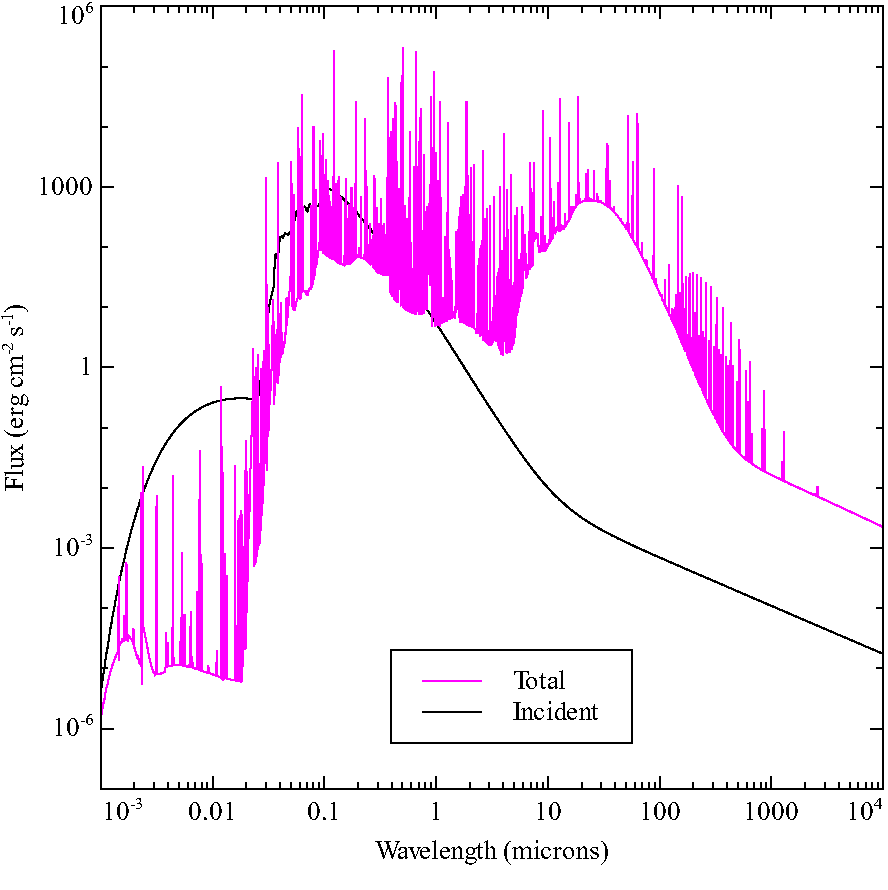
\includegraphics[clip=on,width=0.8\columnwidth,height=0.8\textheight,keepaspectratio]{orion_hii_pdr_pp_con}
\end{center}
\caption{The incident (smooth) and emitted spectrum contained in the
\cdFilename{orion\_hii\_pdr\_pp.con} file.  The
x-axis is the wavelength in microns and
the y-axis gives $vf_v$ [\ergpscmps ].  This is produced by the
\cdCommand{save continuum} command.}
\label{fig:orion_hii_pdr_pp_con}
\end{figure}

\cdFilename{orion\_hii\_pdr\_pp.ovr} is produced
by the \cdCommand{save overview} command.  It gives
the electron temperature and density, the hydrogen density, the heating
rate, and the ionization distribution of H, He, C, and O.
Figure \ref{fig:hydrogen_structure} shows the hydrogen ionization
and chemical structure as given in this file.
The x-axis gives the log of the depth into the cloud in cm.
The y-axis gives the log of the fraction of hydrogen in the form of H$^+$,
H$^0$, and H$_2$.
The hydrogen ionization
front occurs at a depth of $\sim 2 \times 10^{17} \rm{cm}$.
There is a small H$^0$ region and the rest of the cloud is mostly \htwo .

\begin{figure}
\begin{center}
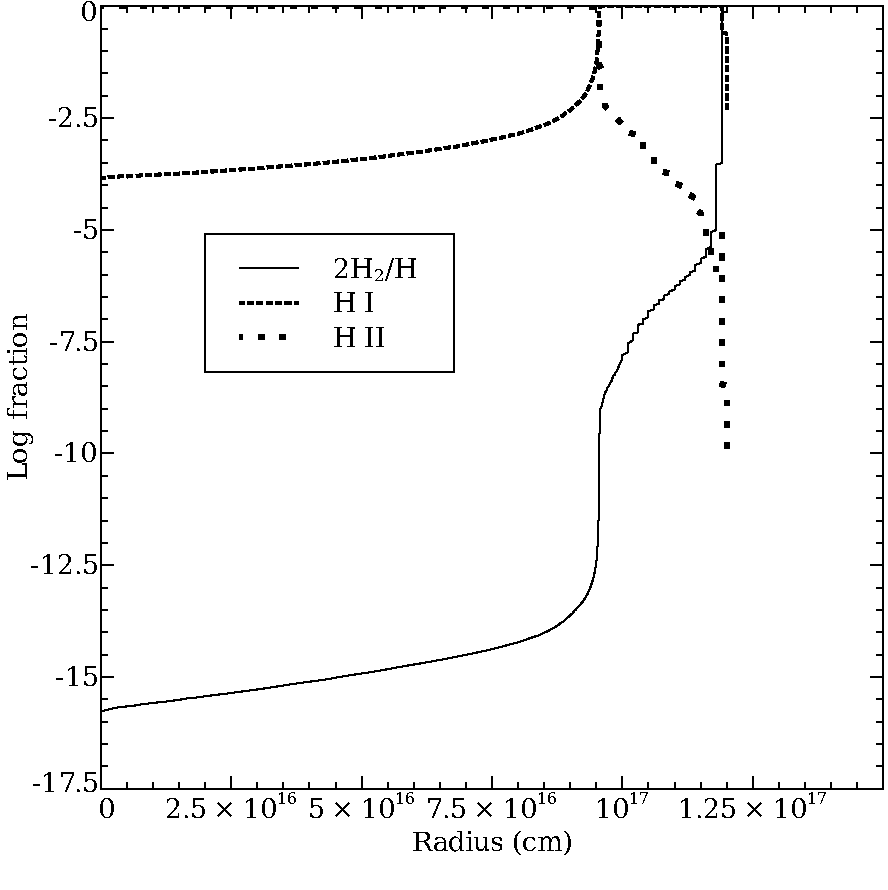
\includegraphics[clip=on,width=0.8\columnwidth,height=0.8\textheight,keepaspectratio]{hydrogen_structure}
\end{center}
\caption{The hydrogen ionization structure.
The x-axis is the depth in cm and the
y-axis gives the log of the fraction of H in H$^+$, H$^0$, and H$_2$.}
\label{fig:hydrogen_structure}
\end{figure}

\cdFilename{orion\_hii\_pdr\_pp.grntem}  gives
temperatures of grains as a function of
depth.
These, together with the electron temperature contained in the
overview file, were used to create Figure \ref{fig:grain_temperature}.
The highest curve
is the electron temperature and is $\sim 10^4 \K$
across the \hplus\ region, falling
to $\sim 500 \K$ in the small \hO\ region,
then to below $100 \K$ in the \htwo\ region.

\begin{figure}
\begin{center}
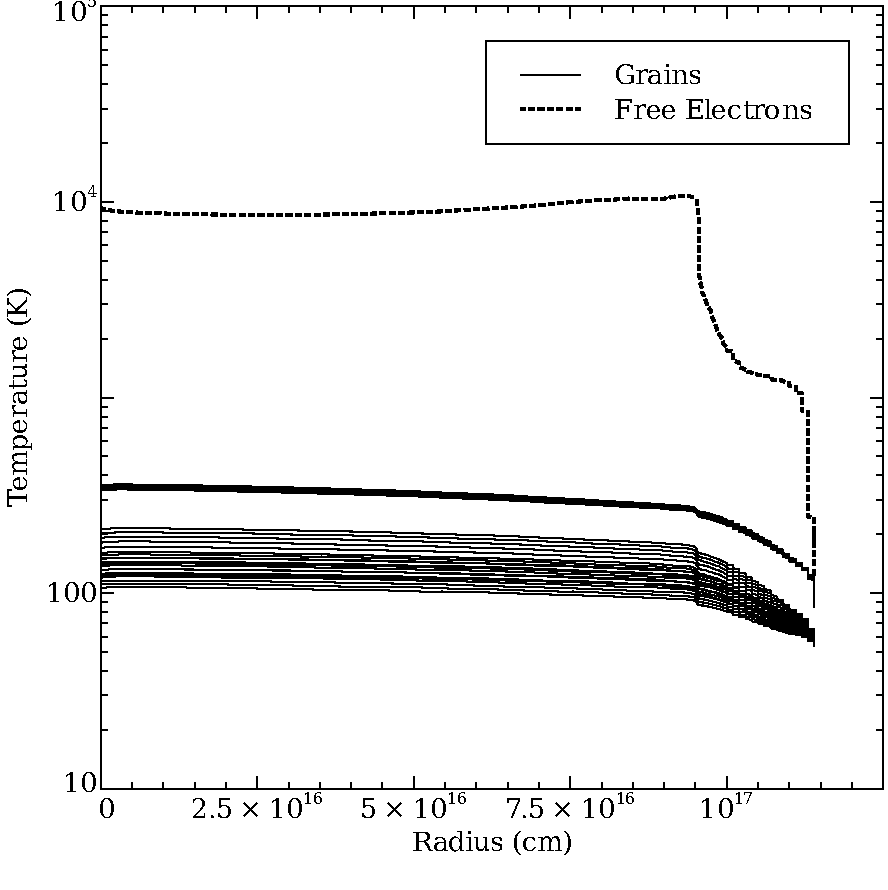
\includegraphics[clip=on,width=0.8\columnwidth,height=0.8\textheight,keepaspectratio]{grain_temperature}
\end{center}
\caption{Temperatures of grains (the lower
cluster of curves) and free electrons
(the higher curve).  They become nearly equal deep in the molecular cloud.
The y-axis is the temperature and the x-axis is the depth into the cloud.}
\label{fig:grain_temperature}
\end{figure}

The calculation includes graphitic and silicate size-resolved grains.
Their temperatures are shown in Figure \ref{fig:grain_temperature}
as the lower cluster of curves.
They have a range of temperatures
$\sim\,$100--200~K across the \hplus\
region and grow cooler in the molecular region.
The gas and dust
temperatures approach one another deep in the molecular cloud.

\cdFilename{orion\_hii\_pdr\_pp.mol} gives molecular
densities as a function of depth
and was used to produce Figure \ref{fig:molecule_structure}.
It also includes several
measures of extinction due to dust.

\begin{figure}
\begin{center}
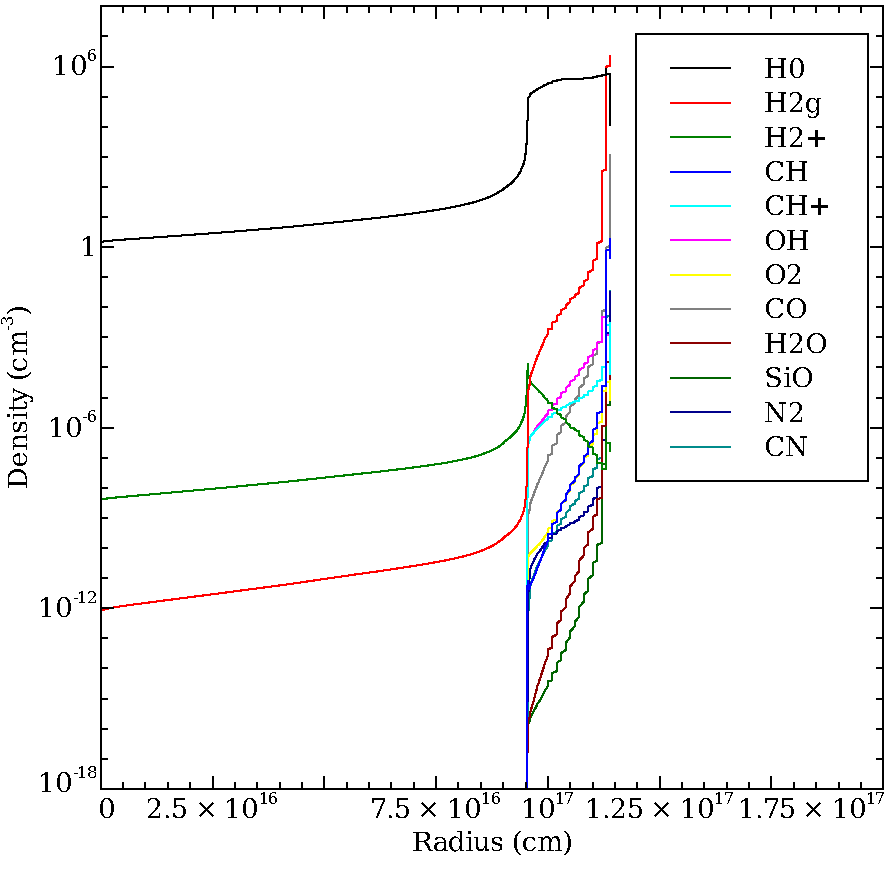
\includegraphics[clip=on,width=\columnwidth,height=0.8\textheight,keepaspectratio]{molecule_structure}
\end{center}
\caption{Densities [cm$^{-3}$] of some of the molecules included in the calculation are shown as a function of depth [cm] into the cloud.}
\label{fig:molecule_structure}
\end{figure}

These are only some of the predictions made by this calculation.
Feel free to explore by changing parameters and assumptions and by adding
other output options.

\subsection{Heads ups for classes of objects}

Simulations of several types of astronomical objects are in the test
suite.  They can be grouped together by the first part of their filename.
The following subsections describe important considerations for setting
up each of these classes of simulations.

\subsubsection{BLR of Active Nuclei}

The density is high enough for free-free absorption of low-energy
radiation to be a significant heating process.
As a result the infrared
continuum can have a surprising effect on the temperature of these clouds.
Extrapolating a reasonable power-law continuum into the infrared may result
in runaway free-free heating.
This, and other practical aspects of BLR
clouds, is discussed in \citet{FerlandBLRCloudReview99}
and in the last two chapters of AGN3.

\subsubsection{NLR of Active Nuclei}

Does dust exist in the ionized gas?  Depletion patterns are not clear,
as discussed by \citet{FergusonEtAl97}.
The NLR is discussed further in the last two chapters of AGN3.

\subsubsection{PDRs of star-forming regions}

It is critical that background cosmic rays, or a source of X-rays, be
included if the simulation is to extend into a molecular cloud.  The
chemistry of cold interstellar matter is driven by a series of ion-molecule
reactions (AGN3 Chapter 8 and Section 11.3).  Chemical interactions between
atoms and ions have smaller activation barriers than interactions between
neutrals so chemistry can occur more quickly when ions are present.  Ions
will not exist if a source of ionization is not present and the chemistry
network may collapse.
Always include the \cdCommand{cosmic ray} and \cdCommand{background} commands.

The \cdCommand{double} command should be
entered if the calculation stops before
the outer edge of the molecular cloud is reached.
See the discussion in Section~\ref{command:double}
on page \pageref{command:double}.

The culture in the PDR modeling community is to treat the PDR as an
isolated phenomenon rather than an extension of the H II region.  Nature
does not do this, but you can force the code to do it by removing all
hydrogen-ionizing radiation from the incident continuum.  This is done with
the \cdCommand{extinguish} command
(see Section~\ref{command:extinguish} on page \pageref{command:extinguish}).

If you do extinguish the hydrogen-ionizing radiation and start a PDR
at that point you will usually find a thin layer of fairly highly-ionized
hydrogen.  This is caused by continuum pumping of the Lyman lines which
then populates the metastable 2\emph{s} term of hydrogen.
That term is then
ionized by the Balmer continuum or $\mathrm{L}\alpha$.
Continuum pumping of Lyman lines
is called ``Case C'' in the ionized-cloud community
\citep{FerlandCaseC99} and is described further in AGN3 Section 11.4.
Classical PDR calculations
do not consider this physics although it is included in Cloudy.
This photoexcitation can be disabled by telling the code
to assume that the Lyman lines are very optically thick
and so are self-shielded.
This is done with
the \cdCommand{Database H-like Lyman pumping off} command.
The \cdCommand{Database H-like Lyman pumping off} command should
not be included in any realistic simulation, which should start with the
\hplus\ region and extend into the PDR as was done by
\citet{Abel2005}.

By default the code will stop when the gas kinetic temperature 
falls below \TEMPSTOPDEFAULT.
PDRs are generally cooler than that.
Many PDR calculations assume that the cloud thickness corresponds
to a visual extinction $A_V$ of 10 mag.
To do this we must tell the code not to stop when the gas becomes
code, and to use this extinction.  This would be done by
\begin{verbatim}
stop temperature off #do not use kinetic temperature as a stopping criterion
stop Av 10  #stop when visual extinction reaches 10 magnitudes
\end{verbatim}

\subsubsection{Galactic nebulae}

Cosmic rays and the ISM background should be included.  Dust is almost
certainly present in the ionized gas and should be included along with
depleted abundances of the refractory elements.
This is important since
the grains extinguish the radiation field, their photoelectrons can heat
the gas, and the gas-phase depletions they cause change
the cooling function \citep{KingdonEtAlGrainEffects95}.
Grains are included by selecting a mix of gas and solids that
includes dust (with one of the \cdCommand{abundances} commands) or by explicitly
including these (with a combination of the \cdCommand{grains},
\cdCommand{abundances}, and \cdCommand{depletion} commands).

\section{How to make this plot}

This section includes examples plots that might be found in research papers on spectroscopy.
It gives an example of the plot, along with an explanation of how to do the calculation
and create it.

\subsection{\htwo\ excitation diagrams}

\htwo\ excitation diagrams show observed or computed level populations 
as a function of the excitation energy in the molecule,
as shown in Figure \ref{fig:H2BFM}.
See AGN3 Chapter 8 and Appendix 4 for background information.
The files used in this example were created with the test suite \citet{Baldwin1991} Orion HII/PDR sim and
are included in the \cdFilename{docs/latex/QuickStart} directory with names starting with
\cdFilename{H2\_BFM}.

\begin{figure}
\begin{center}
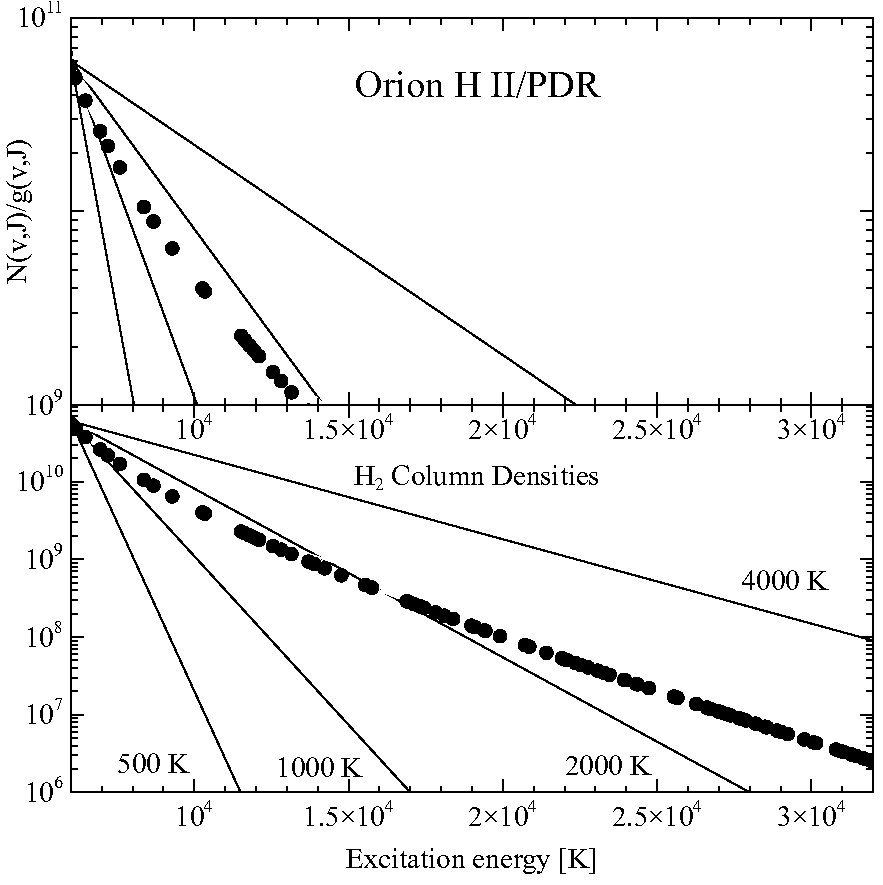
\includegraphics[scale=0.5]{H2_BFM}
\end{center}
\caption{Predicted \htwo\ column densities are shown as a function of excitation energy for
the \citet{Baldwin1991} Orion  \hii\ - PDR model.}
\label{fig:H2BFM}
\end{figure}

Run a simulation that includes the large \htwo\ molecule (with the \cdCommand{atom H2} command)
and include the \cdCommand{save H2 column densities} command.
The first line of the \cdCommand{save} output file gives column headers.
The next three lines give the ortho, para, and total \htwo\ column density,
which we don't need here.
The remaining lines give the column densities and excitation energies for all levels
in the ground electronic state of \htwo.

Import the output of the \cdCommand{save H2 column densities} command into Veusz.
In the import data dialogue specify that the data are tab delimited and to ignore the first three
rows after the header.
Import the rest of the data.

Create an x-y plot and choose column three, the excitation energy in K, as the x-axis.
Choose \cdCommand{colden/stat wght} as the y-axis.
We divide by the statistic weight to avoid having the data jump up and down on the plot
by a factor of three due to the ortho/para distinction.
For plot formatting, choose no line (set line color to while) and use a symbol for the points.
Make the y-axis a log but leave x as linear.

Choose an x-axis range to suite your observations.  The range $5\e3~\K - 3\e4~\K$ includes
most levels that can be detected in the 2~$\mu$m window.

Next we need to add lines indicating the excitation temperature.  
It is easiest to use a spreadsheet to create pairs of points to define this line.
Export this data into a tab delimited file so that Veusz can read it.
Import it into Veusz as a new data set.

To convert observations of \htwo\ lines into column densities you need to divide the observed line by 
a ratio of atomic constants.

\bibliographystyle{plainnat}
\bibliography{../common/bibliography2}

\pagebreak
\appendix
%\documentclass [12pt]{article}
%\usepackage{hyperref}
%\usepackage{fullpage}
%\usepackage{graphicx}

% !TEX root = QuickStart.tex

%\begin{document}

%\maketitle

%\vspace{4in}

%\includegraphics[clip=on,width=\columnwidth,height=0.8\textheight,keepaspectratio]{logo2.png}

%\pagebreak

\section{Veusz Cookbook}
\label{sec:VeuszCookbook}

Most of the plots in this Guide were created with Jeremy Sanders' Veusz plotting package.
Veusz is an open-source and runs on Windows, Mac OS X,
and Linux. Veusz can be downloaded from \url{https://veusz.github.io/}. What follows are a few recipes for basic Cloudy plotting tasks that will get you started with Veusz. For more information, see the Veusz manual at \url{https://veusz.github.io/help-support/}. 
This document assumes that you are using Veusz 1.6 or later.

\subsection{Steps to Import data}

There is an important distinction in this step.
If you create an ``unlinked data set'' Veusz will make your data part of the
Veusz plot file. 
This is good if you want a single self-contained file.
If you create a ``linked data set'' the plot will be linked to the original
data file.  If you update the data file the plot will be updated with no further work.

Veusz does not read spreadsheet files directly.
If you work with your data in a spreadsheet you should save the
data in a field-delimited format.
CSV (comma separated values) or tabs are good choices.

\textbf{Heads up:} Data files created by Cloudy have a first line with 
column headings for the data that follow. These headings have spaces and 
special characters (/, + , -, {\_}, etc.). If you encounter problems with 
Veusz not being able to open files with unlinked data sets, removing 
these characters from your data and re-importing may fix the problem.

\begin{enumerate}
\item Click ``Data''
\item Select ``Import''
\item Choose the file that contains your data clicking ``Browse'' and selecting the file
\item If the data is delimited, select the ``CSV'' tab.
\item Under the ``File Preview'' box select the correct delimiter
\item At the bottom, you have the option to link the dataset to the original file.
\item Click ``Import'' and each column of your data will be saved in a dataset designated by the column heading.
\item Click ``Close''
\end{enumerate}

\subsection{Steps to plot your data (XY points)}

\begin{enumerate}
\item Click ``Insert''
\item Select ``Add xy'' : xy1 will be created in the top white box on the left (Editing Box)
\item The middle box (properties box) on the left side gives the properties of the xy1 pointset
\item In the properties box, click the blue down arrow to the right of ``X data''
\item Select the dataset that you want to appear on the x-axis
\item Repeat steps 4 and 5 for the ``Y data''
\end{enumerate}

\subsection{Steps to Export Plot to PDF}

\begin{enumerate}
\item Click ``File''
\item Select ``Export''
\item Choose the file location with the ``where'' drop down.
\item Click the blue down arrow to the right of the ``Files of Type'' (at the bottom)
\item Choose ``Portable Document Format (*.pdf)''
\item Choose the destination and file name then click ``Save''
\end{enumerate}

\subsection{Change From Points and Line (default) to Line only}

\begin{enumerate}
\item With the desired pointset selected in the Editing Box, select the ``Main'' tab in the Formatting Box (bottom on the left).
\item Click the blue down arrow on the ``Marker'' drop down box
\item Select ``none''
\end{enumerate}

\subsection{Add x-axis title:}

\begin{enumerate}
\item Select ``X'' (of the ``axis'' type) in the Editing Box
\item Enter the desired title for the x-axis in the ``Label'' textbox inside the Properties Box
\end{enumerate}

\subsection{Add y-axis title:}

\begin{enumerate}
\item Select ``Y'' (of the ``axis'' type) in the Editing Box
\item Enter the desired title for the y-axis in the ``Label'' textbox inside the Properties Box
\end{enumerate}

\subsection{Add a second plot:}

\begin{enumerate}
\item Repeat the Steps to plot your data (XY points)
\end{enumerate}

\subsection{Change Line Properties:}

\begin{enumerate}
\item Select the desired pointset in the Editing Box
\item Click the second tab called ``Plot line'' in the Formatting Box
\item In this tab one can change the color, width, style, and transparency of the line for the selected pointset.
\end{enumerate}

\subsection{Adding a Key or Legend:}

\begin{enumerate}
\item Click ``Insert''
\item Select ``Add Key'' -- This will create a blank key/legend box that can be dragged and dropped.
\item Select a pointset from the Editing Box
\item In the Properties Box, enter the text to appear in the key/legend box in the textbox called ``Key text''
\end{enumerate}

\subsection{Create a 2D dataset (Needed for contour or image graphs):}

\begin{enumerate}
\item Ensure that your individual data columns are already imported
\item Click ``Data''
\item Select ``Create 2D''
\item Type in a name for your 2D dataset in the ``Name'' textbox
\item Ensure that the middle option, ``From x, y, and z {\ldots}'', is selected in the ``Method of Creating Dataset'' Box.
\item In the ``Values'' section, choose the desired x, y, and z individual datasets
\item Click ``Create'' -- It should tell you that the dataset was created at the bottom of the form.
\item Click ``Close''
\end{enumerate}
	
\subsection{Create a Contour Plot:}

\begin{enumerate}
\item Click ``Insert''
\item Select ``Add contour''
\item In the Properties Box, select the desired 2D dataset
\end{enumerate}

Veusz automatically chooses contours. It is possible to change the number of 
contours by changing the ``Number Levels'' property. Changing the 
``Scaling'' property changes the way that the contour levels are chosen. 
If the contours are chose automatically, it is important to
specify the ``min'' and ``max'' contours.

\subsection{Set Contour Levels Manually:}

\begin{enumerate}
\item Ensure that the desired contour set is selected in the Editing Box.
\item In the Properties Box, change the ``Scaling'' property to ``Manual''
\item Enter the desired contour levels in the ``Manual Levels'' textbox separated by commas.
\end{enumerate}

\subsection{Add contour labels:}

\begin{enumerate}
\item Click on the 2$^{nd}$ tab in the Formatting Box, called ``Contour labels''
\item Uncheck the ``Hide'' checkbox
\item The font, color, and size can also be adjusted here
\end{enumerate}

\subsection{A bit about contour plots:}

With a contour pointset selected, the Formatting Box contains 5 tabs. The 
first tab, called ``Main formatting'', only allows you to hide the contours.
The next tab over is called ``Contour Labels''. 
Here you can adjust the numerical labels for the contours.

The third tab from the left is called ``Contour Lines''. By default, there is one line style. 
This means that all of the contour lines will have the properties set by this line style. 
The ``Add''button will add a new line style to the list. With 2 line styles, 
the top line style will be applied to the lowest contour line. The second line style 
will be applied to the next lowest contour. The next contour line will then 
take the properties of the top line style. Each successive contour line will 
continue to cycle between the two available line styles. The ``Delete'' 
button deletes the lowest line style on the list. The checkbox to the right 
of the line style properties hides the contour lines that are described by 
the given line style.

The fourth tab is called ``Contour Fill''. It works just like the ``Contour Lines'' tab except
that it fills in the contour areas with different fillers (e.g. solid, vertical lines, etc.). It is also possible
to adjust the color of the fillers.

The fifth tab is ``Sub-contour Lines''. This tab allows you to add a specific number of contour sections evenly spaced between the defined
contour lines. The number of sections to add in between each defined contour line is set by the ``Levels'' textbox. The number of sub-contour lines that will appear between each defined contour is the number in the ``Levels'' textbox minus one. The ``Line Style'' section
of this tab works the same way as the ``Contour Lines'' and ``Contour Fill'' tab. Note that you have to uncheck the ``Hide'' checkbox to view
the sub-contours.

\subsection{Filled contour maps}

A variety of filled contour maps are available.  
Do insert / image and then select a 2D dataset.
Several color and grey-scales are available.

If you want both the contour lines and the filled image then the contours must be
on top of the filled contour.  

Figure \ref{fig:grid_extreme} shows an example, 
taken from the \cdCommand{grid\_extreme} test in the slow test suite.
This uses the spectrum2 colormap and goes from red to blue as the
temperature goes from low to high values.

\begin{figure}
\begin{center}
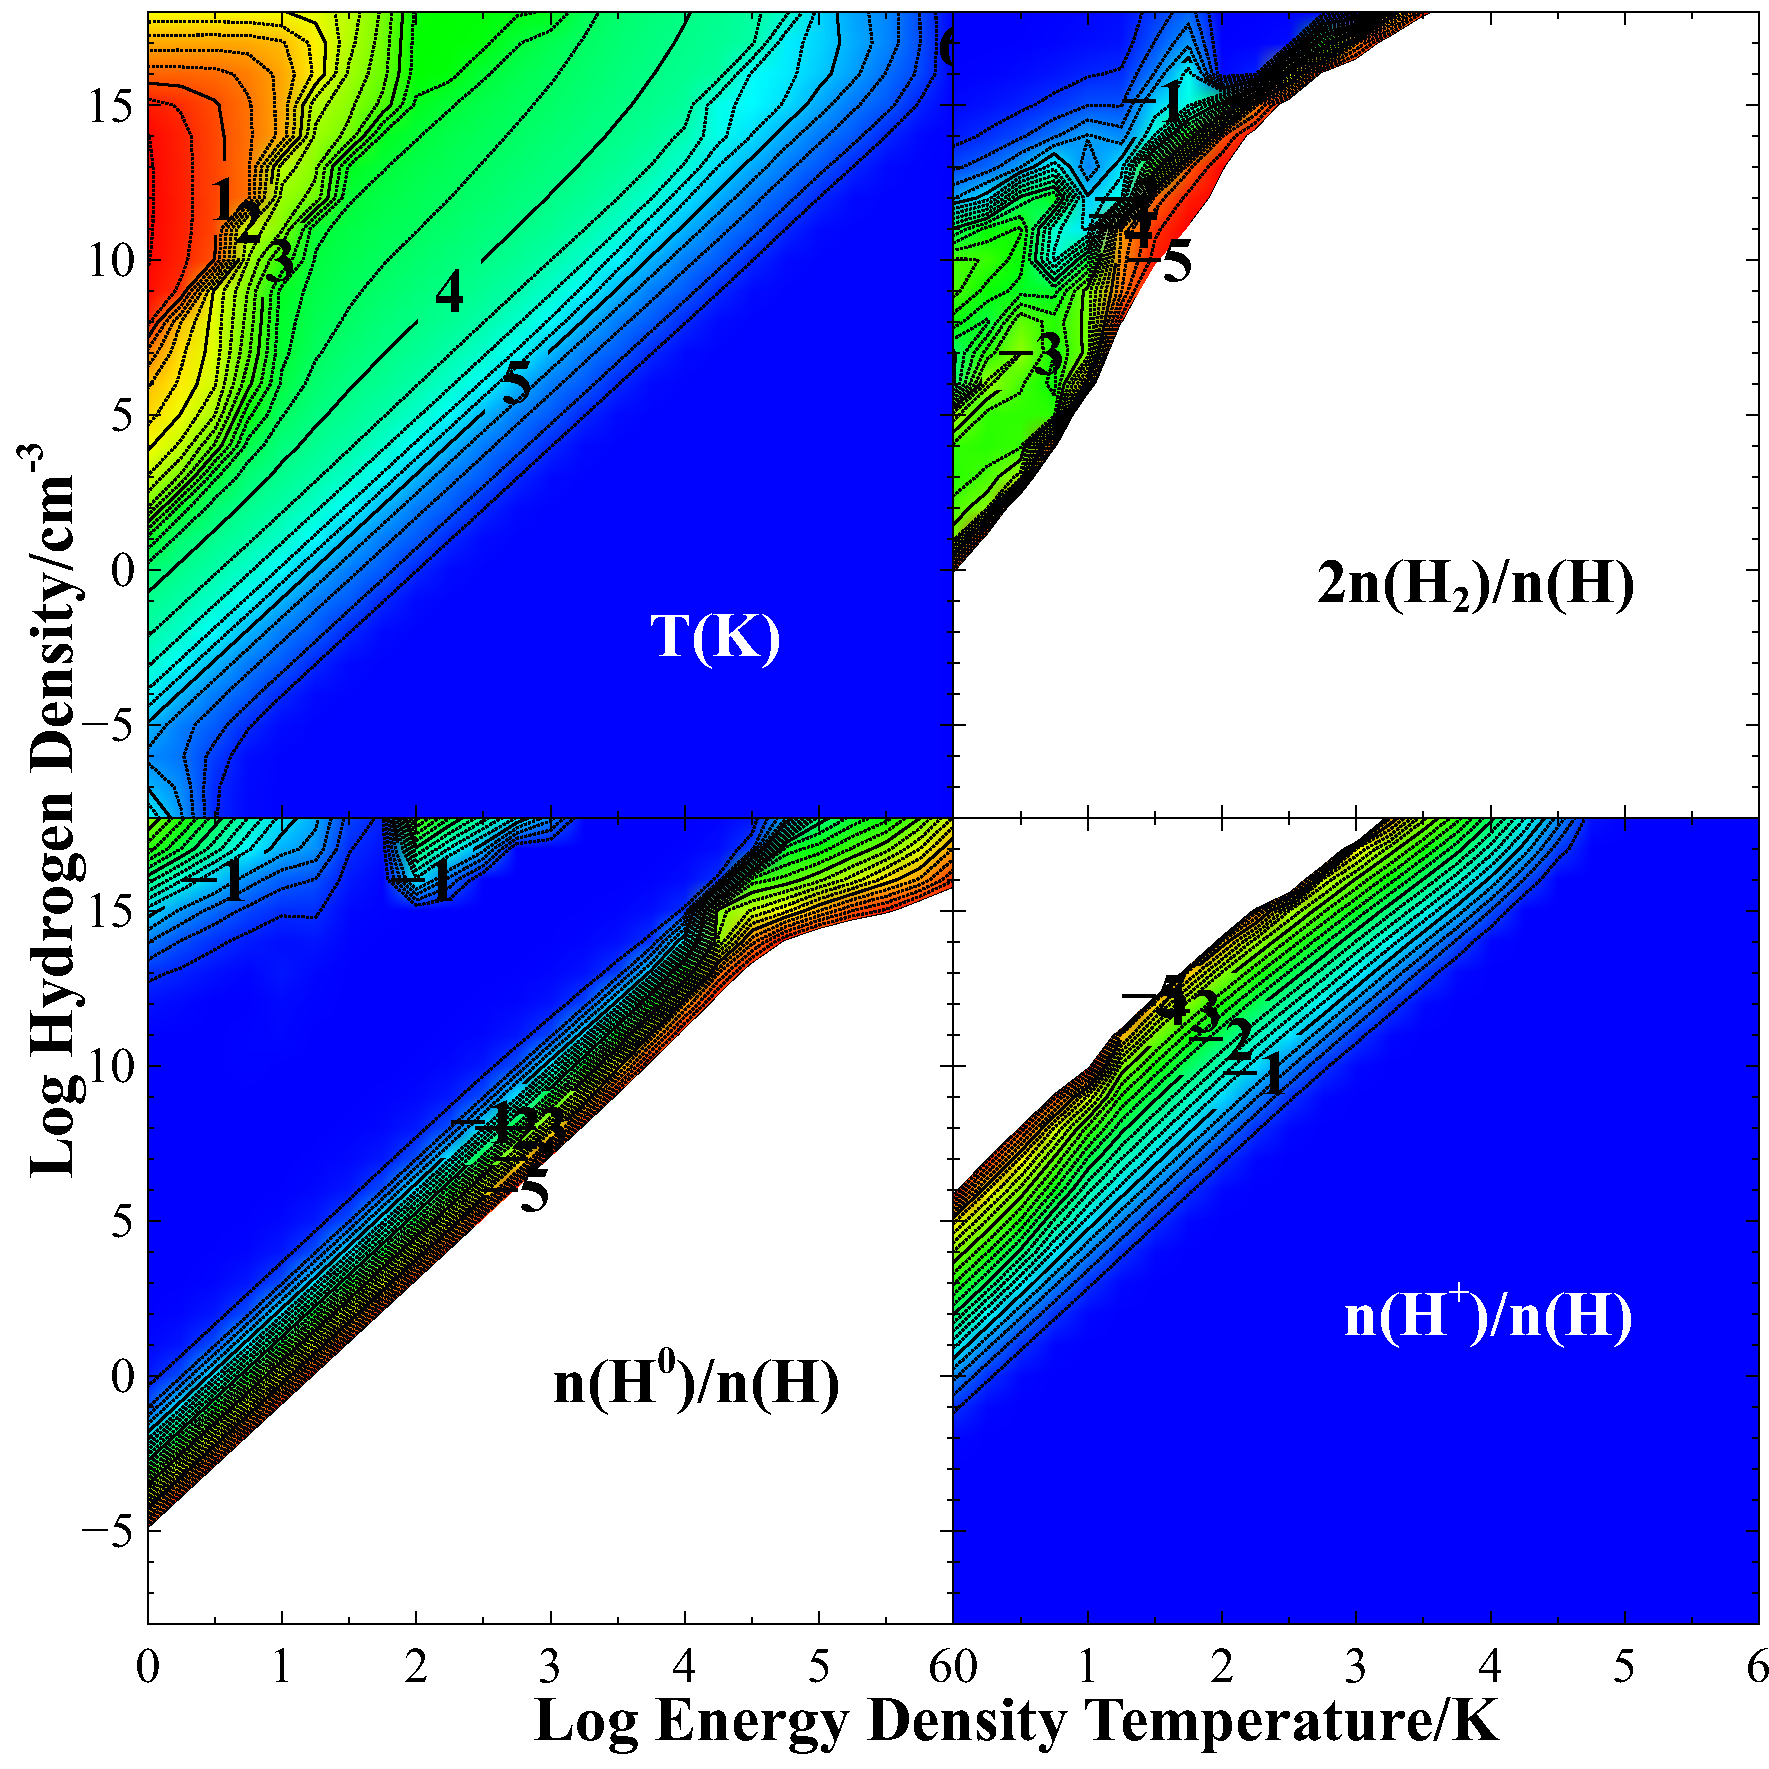
\includegraphics[clip=on,width=0.9\columnwidth,height=0.7\textheight,keepaspectratio]{grid_extreme}
\end{center}
\caption{This shows physical conditions over a very broad range of hydrogen density 
and energy-density temperature.  
The log of the electron kinetic temperature is shown in the upper left,
and hydrogen ionization and molecular fractions in the remaining panels.
The gas goes to the Compton temperature in the 
upper left corner of each panel, is in the blackbody limit across the top, and is close to LTE 
across the right-hand edges of the figure.}
\label{fig:grid_extreme}
\end{figure}

\subsection{Multiple graphs}

The graphs are made out of widgets that can be placed inside each other, e.g. 
graphs can be placed in pages, and different types of plotting widgets, e.g. xy or function, 
can be placed in graphs. 
You can also place graphs within a grid widget to get an arrangement of separate graphs.

Figure \ref{fig:orion_hii_pdr_pp} shows an example, 
taken from the Orion HII region / PDR simulation, of a nested plot.


\begin{figure}
\begin{center}
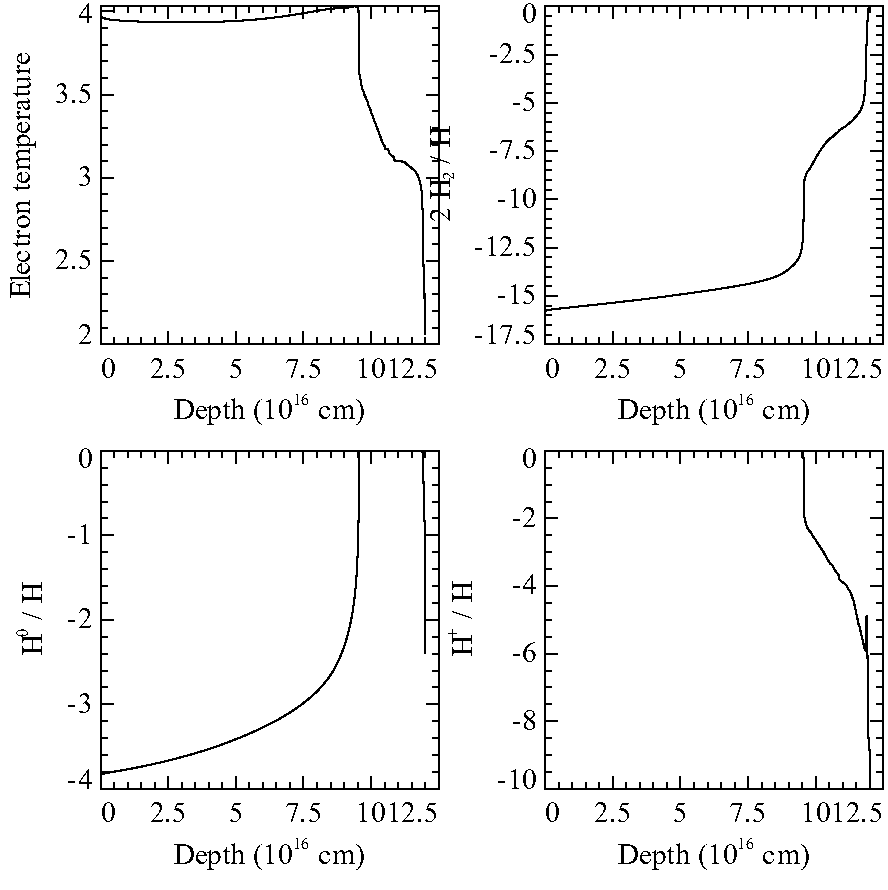
\includegraphics[clip=on,width=0.8\columnwidth,height=0.8\textheight,keepaspectratio]{orion_hii_pdr_pp}
\end{center}
\caption{The electron kinetic temperature, and fractions of H in H$_2$,
H$^0$, and H$^+$, are shown as a function of depth into the 
Orion H II region / PDR.}
\label{fig:orion_hii_pdr_pp}
\end{figure}


\subsection{Documenting your work}

The Properties widget includes a Notes field that can be used to keep a history of the 
data behind a plot.
This is useful so that you can come back to a project after some time and recover
the history of the work leading up to a result or the location of the helper files that were used
along the way.

%\end{document}


\end{document}


